 % -*- root: ../thesis.tex -*-

\chapter{Tensors}%
\label{chap:tensors}


\todo{The $A\ind{l}$ notation is used for two different things here.}

The theoretical and numerical study of many-body quantum systems is severely hindered by the \emph{curse of dimensionality}, which in this context refers to the exponential growth of the Hilbert space of quantum states w.r.t.\ the number of constituents.
However, many realistic systems do not exhibit this pathological complexity and can be described efficiently in terms of \emph{tensor networks}~\cite{}.
An especially simple but important special case of tensor networks is known under names such as \emph{finitely correlated states}~\cite{Fannes_1992_Finitely} or \emph{matrix-product states} (MPS)~\cite{Garcia_2006_Matrix,Verstraete_2008_Matrix,Orus_2014_Practical}.
\todo{Check this!}
Examples for quantum states that can be efficiently described as MPS include W-, GHZ-, and cluster states.
More generally, low energy states of one-dimensional gapped Hamiltonians with local interactions have an efficient MPS description and vice versa~\cite{}.
Here, \quotes{efficient description} refers to the fact that the number of parameters required to describe such a state scales polynomially in the number of subsystem.

The question we are attempting to answer in this chapter is whether such MPS can be efficiently reconstructed from few linear measurements\footnote{%
  Note that since we assume a linear measurement model, the results of this section do not apply to the problem of estimating pure quantum states.
  We use the term \quotes{matrix product state} to not only refer to quantum states, but to general tensors in the MPS format.
}.
More precisely, we provide evidence that the number of measurements required to recover a MPS is related to its intrinsic complexity -- and hence, scales polynomially in the number of constituents -- although its Hilbert space is exponentially large.
\todo{Two fold: compressed sensing and scalable MMLE}
This work is a natural extension of \emph{low-rank matrix recovery}, which formed the foundation of the results in \cref{chap:phaselift}, to higher-order tensors.\\
\todo{tensors -> higher order, rank}

This chapter is structured as follows:
In \cref{sec:tensors.mps}, we introduce the MPS tensor format.
\Cref{sec:tensors.als} reports on work in progress, which is concerned with recovering MPS from few linear measurements using an \emph{Alternating Least Squares} (ALS) algorithm.
Finally, in \cref{sec:tensors.mpnum} we present the software library \mpnum dealing with tensors in MPS representation.
\mpnum was developed as part of this work to facilitate numerical computations in a user friendly and reusable manner.


\subsection*{Relevant publications}
\begin{itemize}
  \item Ž.\ Stojanac, D.\ Suess, M.\ Kliesch: \textit{On the distribution of a product of N Gaussian random variables}, Proceedings Volume 10394, Wavelets and Sparsity XVII; 1039419 (2017)
  \item Ž.\ Stojanac, D.\ Suess, M.\ Kliesch, \textit{On products of Gaussian random variables}, arXiv:1711.10516
  \item D.\ Suess, M.\ Holzaepfel, \textit{mpnum: A matrix product representation library for Python}, Journal of Open Source Software, 2(20), 465 (2017)
\end{itemize}
%%%%%%%%%%%%%%%%%%%%%%%%%%%%%%%%%%%%%%%%%%%%%%%%%%%%%%%%%%%%%%%%%%%%%%%%%%%%%%%%
\section{Matrix Product States}%
\label{sec:tensors.mps}

Tensors are a generalization of vectors and matrices.
Although there is a coordinate-free definition for tensors in terms of multi-linear functionals~\cite{Browder_2012_Mathematical}, we are going to identify a tensor with its coordinate representation here.
\todo{Also no distinguishing co/contravariant indices -> euclidean}
A complex tensor of order $N$ is an element $X \in \Complex^{d_1 \times \cdots \times d_N}$ and the $d_i$ are called \emph{local dimensions}.
Hence, a vector is a tensor of order 1 and a matrix is a tensor of order 2.
For the sake of simplicity, we assume that $d_1 = \cdots = d_N$ throughout this chapter.



\subsection{Graphical Notation}
\label{sub:mps.graphical_notation}

Since formulas with higher-order tensors may become incomprehensible due to the large amount of indices necessary, we introduce a common graphical notation~\cite{Orus_2014_Practical,Bridgeman_2017_HandWaving}.
A tensor $X \in \Complex^{d^N}$ is represented by a geometric shape with legs attached, one for each index.
For example, consider the case $N = 3$, then
\[
  X_{i,j,k}
  =
  \begin{tikzpicture}[baseline=-.5ex]
    \tensor{{S=3, tensor_width=2, len_vertical_legs=0.5}}
    \node at (X) {$X$};
    \node [anchor=north] at (X_S1e) {\small $i$};
    \node [anchor=north] at (X_S2e) {\small $j$};
    \node [anchor=north] at (X_S3e) {\small $k$};
  \end{tikzpicture}
  .
\]
A variable written next to a leg fixes the corresponding index to the given value, while an anonymous tensor leg represents an unmatched index.
In the following, we will make use of the following notation for an unmatched index inspired by Python's and Matlab's syntax:
Given above $X \in \Complex^{d^3}$, we define the slice $X_{:,j,:} \in \Complex^{d^2}$ by
\[
  \label{eq:mps.slicing}
  X_{:,j,:}
  =
  \begin{tikzpicture}[baseline=-.5ex]
    \tensor{{S=3, tensor_width=2, len_vertical_legs=0.5}}
    \node at (X) {$X$};
    \node [anchor=north] at (X_S2e) {\small $j$};
  \end{tikzpicture}
  .
\]
For the components, we have the slightly cumbersome equality $\left(X_{:,j,:}\right)_{i,k} = X_{i,j,k}$.
The advantage of this graphical notation becomes clear once we express tensors composed of other tensors by operations such as index contraction or tensor products:
\begin{description}[font=$\bullet$\ \scshape\bfseries]
  \item[Contractions] are indicated by joining two legs, e.g.\ for matrices $A, B \in \Complex^{d \times d}$ their product $AB$ is written as
    \[
      \begin{tikzpicture}[baseline=-.5ex]
        \tensor{{W=1, E=1, tensor_name='AB'}}
        \node at (AB) {$AB$};
      \end{tikzpicture}
      =
      \begin{tikzpicture}[baseline=-.5ex]
        \tensor{{W=1, E=1, tensor_name='A'}}
        \node at (A) {$A$};
        \tensor{{W=1, E=1, tensor_name='B', x=1.25}}
        \node at (B) {$B$};
      \end{tikzpicture}
      :=
      \sum_k
      \left(
      \begin{tikzpicture}[baseline=-.5ex]
        \tensor{{W=1, E=1, tensor_name='A'}}
        \node at (A) {$A$};
        \node[anchor=west] at (A_E1e) {\small $k$};
        \tensor{{W=1, E=1, tensor_name='B', x=2.5}}
        \node at (B) {$B$};
        \node[anchor=east] at (B_W1e) {\small $k$};
      \end{tikzpicture}
      \right)
    \]

  \item[Tensor products] correspond to drawing two tensors side by side, e.g.\ for $x, y \in \Complex^d$ their tensor product $x \otimes y$ is written as
    \[
      \begin{tikzpicture}[baseline=-.5ex]
        \tensor{{S=2, tensor_width=1.5, tensor_name='xy'}}
        \node at (xy) {$x \otimes y$};
      \end{tikzpicture}
      =
      \begin{tikzpicture}[baseline=-.5ex]
        \tensor{{S=1, tensor_name='x'}}
        \node at (x) {$x$};
        \tensor{{S=1, tensor_name='y', x=1.25}}
        \node at (y) {$y$};
      \end{tikzpicture}
    \]

  \item[Grouping] indices -- that is the canonical identification $\Complex^{d_1} \otimes \Complex^{d_2} \cong \Complex^{d_1 d_2}$ -- is indicated by merging two or more legs together.
    \[
      \tikz[baseline=-.5ex]{\mpa{2}{{W=3, virtual=2, E=1}}}
      \cong
      \begin{tikzpicture}[baseline=-.5ex]
        \tensor{{W=1, E=1, len_horizontal_legs=0, tensor_name='A'}}
        \tensor{{W=1, E=1, len_horizontal_legs=0, tensor_name='B', x=1.25}}
        \draw[line width=2pt] (A_W1) -- +(-0.25,0);
        \draw[line width=1.5pt] (A_E1) -- (B_W1);
        \draw (B_E1) -- +(0.25,0);
      \end{tikzpicture}
      \label{eq:tensors.intro.grouping}
    \]
    This operation is often used in numerical implementations of tensor network algorithms as it reduces most tensor operations to standard matrix  operations.
    For example, the twofold contraction on the left hand side of \cref{eq:tensors.intro.grouping} is converted to a matrix multiplication on the right hand side.
    In the following, we often implicitly perform grouping on neighbouring tensor legs.
\end{description}



\subsection{MPS tensor representation}%
\label{sub:mps.tensor_representation}

The tensor representation we are interested in has been established in quantum physics independently under the names \emph{finitely correlated states}~\cite{Fannes_1992_Finitely} and \emph{matrix-product states}~\cite{Klumper_1991_Equivalence,Kluemper_1992_Groundstate}.
Subsequently, it has been rediscovered in other contexts:
It is known under the guise of the \emph{density matrix renormalization group}~\cite{White_1992_Density,Schollwoeck_2011_DensityMatrix} in condensed matter physics.
Furthermore, the MPS representation is also known as a special case of the \emph{Hierarchical Tucker} tensor format~\cite{Hackbusch_2012_Tensor,Grasedyck_2010_Hierarchical} and under name \emph{tensor-train}~\cite{Oseledets_2011_TensorTrain} in the applied math community.
However, similar structures have been known for much longer in the form of \emph{deterministic finite automata}~\cite{Hopcroft_2014_Introduction} and \emph{hidden Markov models}~\cite{Cappe_2006_Inference}.

\todo{More motivation?}

To introduce the MPS representation, consider a tensor $X \in \Complex^{d^N}$.
By splitting off the first index, grouping the remaining $N-1$ indices, and performing a SVD on the resulting matrix, we can factor $X$ into three parts
\[
  \begin{tikzpicture}[baseline=-.5ex]
    \tensor{{S=4, tensor_width=3}}
    \node (X) {$X$};
    \draw[dashed] (-.6,-.8) -- (-.6, .8);
  \end{tikzpicture}
  =
  \begin{tikzpicture}[baseline=-.5ex]
    \tensor{{S=1, E=1, x=-3.3, tensor_name='L'}}
    \node at (L) {$M\ind{1}$};
    \tensor{{W=1, E=1, x=-2.1, tensor_name='lambda', tensor_style='tensornode, rounded corners=0.375cm, fill=red!30'}}
    \node at (lambda) {$\Lambda\ind{1}$};
    \tensor{{W=1, S=3, tensor_width=2.5, tensor_name='R'}}
    \node (R) {$\tilde R_{N-1}$};
  \end{tikzpicture}
\]
where $M\ind{1}$ denotes the left-singular vectors, $\Lambda\ind{1}$ the diagonal matrix composed of the singular values $\lambda\ind{i}$, and $\tilde R_{N-1}$ the left-singular vectors after the index-grouping has been reversed.
For convenience, we contract the singular values with the remainder $\tilde R_{N-1}$ and obtain
\[
  \begin{tikzpicture}[baseline=-.5ex]
    \tensor{{S=4, tensor_width=3}}
    \node (X) {$X$};
  \end{tikzpicture}
  =
  \begin{tikzpicture}[baseline=-.5ex]
    \tensor{{S=1, E=1, x=-2.1, tensor_name='L'}}
    \node at (L) {$M\ind{1}$};
    \tensor{{W=1, S=3, tensor_width=2.5, tensor_name='R'}}
    \node (R) {$R_{N-1}$};
  \end{tikzpicture}
\]
This procedure can now be iterated by performing the same steps on $R_{N-1}$:
\begin{align}
  \begin{tikzpicture}[baseline=-.5ex]
    \tensor{{S=4, tensor_width=3}}
    \node (X) {$X$};
    \draw[dashed] (-.6,-.8) -- (-.6, .8);
  \end{tikzpicture}
  &=
  \begin{tikzpicture}[baseline=-.5ex]
    \tensor{{S=1, E=1, x=-2.1, tensor_name='L'}}
    \node at (L) {$M\ind{1}$};
    \tensor{{W=1, S=3, tensor_width=2.5, tensor_name='R'}}
    \node (R) {$R_{N-1}$};
    \draw[dashed] (-.3,-.8) -- (-.3, .8);
  \end{tikzpicture}\\
  &=
  \begin{tikzpicture}[baseline=-.5ex]
    \mpa{{1,2}}{{S=1, E=1, x=-3.1, tensor_name='L'}}
    \node at (L_1) {$M\ind{1}$};
    \node at (L_2) {$M\ind{2}$};
    \tensor{{W=1, S=2, tensor_width=2}}
    \node (R) {$R_{N-2}$};
    \draw[dashed] (0,-.8) -- (0, .8);
  \end{tikzpicture}\\
  &=
  \begin{tikzpicture}[baseline=-.5ex]
    \mpa{4}{{S=1, tensor_name='L'}}
    \node at (L_1) {$M\ind{1}$};
    \node at (L_2) {$M\ind{2}$};
    \node at (L_3) {$M\ind{3}$};
    \node at (L_4) {$M\ind{4}$};
  \end{tikzpicture}
  \label{eq:mps.matrix_product}
\end{align}
This yields a representation of $X$ in terms of the \emph{local tensors} $M\ind{l}$.
The above algorithm for computing the local tensors is referred to as TT-SVD in \cite{Oseledets_2011_TensorTrain}.
In the following, we identify the index order as follows:
\[
  M\ind{l}_{i,j,k} =
  \begin{tikzpicture}[baseline=-.5ex]
    \tensor{{W=1, S=1, E=1}}
    \node at (X) {$M\ind{l}$};
    \node [anchor=east] at (X_W1e) {\small $i$};
    \node [anchor=west] at (X_S1e) {\small $j$};
    \node [anchor=north] at (X_W1e) {\small $k$};
  \end{tikzpicture}
\]
The horizontal, contracted legs corresponding to the indices $i$ and $k$, are often referred to as \emph{bond} or \emph{virtual legs} and the vertical, unmatched ones corresponding to $j$ are referred to as \emph{physical} legs.
By fixing each physical leg to some value $k_l$ in \cref{eq:mps.matrix_product}, we see that each component of $X$ is given by product of $N$ matrices
\[
  \label{eq:mps.local_matrices}
  M\ind{l}_{k_l} := M\ind{l}_{:,k_l,:},
\]
hence the name \quotes{matrix-product representation}.

%%%%%%%%%%%%%%%%%%%%%%%%%%%%%%%%%%%%%%%%%%%%%%%%%%%%%%%%%%%%%%%%%%%%%%%%%%%%%%%%
\begin{figure*}
  \centering
  \begin{tikzpicture}
    \tensor{{S=4, tensor_name='psi', tensor_width=3, tensor_height=1,
             len_vertical_legs=.5, x=-2.5}}
    \node at (psi) {$X_{ijkl}$};

    \node at (0,0) {\Huge $=$};

    \begin{luacode*}
      local indices = {'i', 'j', 'k', 'l'}
      -- local bond_indices = {'a', 'b', 'c'}

      mptikz.draw_mpa(4, {S=1, tensor_name='A', tensor_width=1, tensor_height=1,
                          len_vertical_legs=.5, len_horizontal_legs=.5, x=1.5})

      for i = 1, 4 do
        t('\\node[anchor=west] at (psi_S%i) {$%s$};', i, indices[i])
        t('\\node[anchor=west] at (A_%i_S1) {$%s$};', i, indices[i])
          t('\\node at (A_%i) {$M\\ind{%i}$};', i, i)
      end

      -- for i =1, 3 do
      --  t('\\node[anchor=north] at (A_%i_E1e) {$%s$};', i, bond_indices[i])
      -- end
    \end{luacode*}

    \draw[pointerline] (psi) -- +(2,-1) node[pointernode] {global tensor};
    \draw[pointerline] (A_2) -- +(1,1) node[pointernode] {local tensor};
    \draw[pointerline] (A_3_E1e) -- +(0.5,1) node[pointernode] {virtual leg};
    \draw[pointerline] (A_3_S1) -- +(-0.5,-0.5) node[pointernode,anchor=east] {physical leg};
  \end{tikzpicture}
  \caption{%
    \label{fig:mps.mps}
    A 4th order tensor in MPS representation with open boundary condition as described in \cref{eq:mps.open_boundary}.
  }
\end{figure*}
%%%%%%%%%%%%%%%%%%%%%%%%%%%%%%%%%%%%%%%%%%%%%%%%%%%%%%%%%%%%%%%%%%%%%%%%%%%%%%%%

So far this construction is exact and completely general, i.e.\ every tensor can be represented in MPS form, but not efficient:
Generically, the SVD in the $i$-th step yields $r_i = \min{d^i, d^{N - i}}$ non-zero singular values $\lambda\ind{i}$, and therefore, the local tensors $M\ind{i}$ have shape $(d, r_{i-1}, r_i)$.
However, suppose that all but $r$ of the singular values in each cut vanish, then we can truncate the local tensor $M\ind{i}$ to shape $(d, r, r)$.
In this case, the number of parameters scales as $\Order(r^2 N d)$ and $X$ can be represented efficiently by matrix products according to \cref{eq:mps.matrix_product}.
Although this assumption may seem overly strict on a first glance, many tensors in our applications of interest are well approximated by such an MPS with small $r$.
The following definition sums up this section so far.

\begin{definition}%
  \label{def:mps.mps}
  A \emph{matrix-product state representation} of a tensor $X \in \Complex^{d^N}$ is defined in terms of a tuple of local tensors $(M\ind{l})_{l \in [N]}$ with $M\ind{l} \in \Complex^{r_{l - 1} \times d \times r_l}$ where $r_0 = r_N$.
  Then, the components of $X$ are given by
  \[
    \label{eq:mps.periodic_boundary}
    X_{i_1,\ldots,i_N} = \tr \left( M\ind{1}_{:,i_1,:}\ \cdots\  M\ind{N}_{:,i_N,:} \right).
  \]
  We say that the MPS representation has \emph{open boundary conditions} if $r_0 = r_N = 1$, otherwise the representation has \emph{periodic boundary conditions}.
\end{definition}

For the sake of simplicity, we restrict our attention to the open boundary case in the following.
In this case, we have
\[
  \label{eq:mps.open_boundary}
  X_{i_1,\ldots,i_N} = M\ind{1}_{i_1}\ \cdots\  M\ind{N}_{i_N},
\]
where we used the shorthand notation from \cref{eq:mps.local_matrices}
As already noted above, the crucial parameter balancing the efficiency of the MPS representation on one hand and its expressive power on the other hand is the size of the virtual legs $r_l$.
This warrants the following definition.

\begin{definition}%
  \label{def:mps.rank}
  Let $(M\ind{l})_{l \in [N]}$ denote an MPS representation with $M\ind{l} \in \Complex^{r_{l - 1} \times d \times r_l}$.
  We call $\max_l r_l$ the (MPS-)\emph{rank} or \emph{bond dimension} of the MPS.
  Furthermore, for any tensor $X$, we define its \emph{MPS-rank} to be the smallest rank of any MPS representation of $X$.
\end{definition}

Note that by~\cite[Thm.\ 2.2]{Oseledets_2011_TensorTrain}, the definition of MPS-rank in \cref{def:mps.rank} agrees with the usual definition using matrications of $X$, and hence, is well defined.
\todo{Fix this}
In contrast to the matrix case, there are multiple inequivalent definitions rank for tensors~\cite{???}.
% Each notion of rank is induced by a tensor representation analogous to the MPS case.
% The choice which format to use in practice is mainly determined by two factors:
% On the one hand, the natural structure of the problem determines, which tensor format yields the most efficient
\\


With the factorization of the tensor $X$ in \cref{def:mps.mps}, we have introduced new virtual degrees of freedom such that the partial trace over them equals $X$.
Clearly, the following gauge transformation leaves \cref{eq:mps.open_boundary} invariant
\begin{align}
  \tilde M\ind{1}_i = M\ind{1}_i R\ind{1},
  \tilde M\ind{N}_i = R\ind{N - 1} M\ind{N}_i, \\
  \tilde M\ind{l}_i = L\ind{l - 1} M\ind{l}_i R\ind{l} \quad (1 < l < N)
\end{align}
provided the (generally non-square) matrices $L\ind{l}$ and $R\ind{l}$ satisfy $L\ind{l} R\ind{l} = \1$ since then
\[
  \begin{tikzpicture}[baseline=-.5ex]
    \mpa{4}{{S=1, tensor_name='A', len_horizontal_legs=0.1}}
    \node at (A_1) {$M\ind{1}$};
    \node at (A_2) {$M\ind{2}$};
    \node at (A_3) {$M\ind{3}$};
    \node at (A_4) {$M\ind{4}$};
  \end{tikzpicture}
  =
  \begin{tikzpicture}[baseline=-.5ex]
    \mpa{{1,4,7,10}}{{S=1,tensor_name='B', len_horizontal_legs=0.1}}
    \node at (B_1) {$M\ind{1}$};
    \node at (B_4) {$M\ind{2}$};
    \node at (B_7) {$M\ind{3}$};
    \node at (B_10) {$M\ind{4}$};
    \mpa{{2,5,8}}{{tensor_name='R', E=1, len_horizontal_legs=0.1, tensor_style='tensornode, fill=red!30'}}
    \node at (R_2) {$R\ind{1}$};
    \node at (R_5) {$R\ind{2}$};
    \node at (R_8) {$R\ind{3}$};
    \mpa{{3,6,9}}{{tensor_name='L', len_horizontal_legs=0.1, tensor_style='tensornode, fill=red!30'}}
    \node at (L_3) {$L\ind{1}$};
    \node at (L_6) {$L\ind{2}$};
    \node at (L_9) {$L\ind{3}$};
  \end{tikzpicture}
\]
As shown in~\cite[Thm. 2]{Garcia_2006_Matrix}, these local transformations on the virtual degrees of freedom are the only possible gauge transformations of the MPS representation.
A number of canonical forms exist that partially fix the gauge~\cite{Garcia_2006_Matrix,Schollwoeck_2011_DensityMatrix,Bridgeman_2017_HandWaving}.
The following definition summarizes the corresponding gauge conditions

\begin{definition}%
  \label{def:mps.canonical}
  We say that a local tensor $M\ind{l}$ is \emph{left-normalized} if it satisfies
  \[
    \sum_k \adj{M\ind{l}_k} M\ind{l}_k = \1 \quad\quad\quad\quad
    \begin{tikzpicture}[baseline=-.5ex]
      \tensor{{W=1,S=1,E=1,tensor_name='A',y=0.5}}
      \tensor{{W=1,N=1,E=1,tensor_name='B',y=-0.5}}
      \draw[tensorleg] (A_W1e) -- (B_W1e);
    \end{tikzpicture}
    =
    \begin{tikzpicture}[baseline=-.5ex]
      \coordinate (A) at (0,0.5);
      \coordinate (B) at (0,-0.5);
      \draw[tensorleg] (A) -- (B);
      \draw[tensorleg] (A) -- +(.5,0);
      \draw[tensorleg] (B) -- +(.5,0);
    \end{tikzpicture}
  \]
  A MPS with all but the rightmost local tensors in left-normalized form is called \emph{left-canonical}.
  Similarly, a \emph{right-normalized} local tensor fulfills
  \[
    \sum_k M\ind{l}_k \adj{M\ind{l}_k} = \1 \quad\quad\quad\quad
    \begin{tikzpicture}[baseline=-.5ex]
      \tensor{{W=1,S=1,E=1,tensor_name='A',y=0.5}}
      \tensor{{W=1,N=1,E=1,tensor_name='B',y=-0.5}}
      \draw[tensorleg] (A_E1e) -- (B_E1e);
    \end{tikzpicture}
    =
    \begin{tikzpicture}[baseline=-.5ex]
      \coordinate (A) at (0,0.5);
      \coordinate (B) at (0,-0.5);
      \draw[tensorleg] (A) -- (B);
      \draw[tensorleg] (A) -- +(-.5,0);
      \draw[tensorleg] (B) -- +(-.5,0);
    \end{tikzpicture}
  \]
  and a \emph{right-canonical} MPS has all local tensors in right-normalized form except for the first.
\end{definition}

The exceptions for the local tensors at the beginning and end of the chain are necessary to accommodate tensors with Frobenius norm different from one.
In practice, we often deal with a mixed left-right-canonical form, e.g.\ in variational algorithms updating one local tensor at a time such as DMRG or the alternating least squares algorithm presented in \cref{sec:tensors.als}.
For these purposes, efficient algorithms exist that transform an MPS to a canonical form~\cite{Schollwoeck_2011_DensityMatrix,Orus_2014_Practical}.
If we neglect transformations that change the bond dimensions, the remaining gauge group is unitary, and hence, computations on canonical MPS are far more stable numerically.\\


We have already emphasized the ability of the MPS representation to represent certain tensors efficiently, i.e.\ with a number of parameters scaling polynomially in the order of the tensor.
One crucial advantage of this tensor format is that it also facilitates efficient arithmetical operations for tensors~\cite{Schollwoeck_2011_DensityMatrix,Orus_2014_Practical}.
In other words, operations such as sums and contractions of MPS are also MPS and the corresponding local tensors can be computed efficiently from the local tensors of the inputs.
For example, consider the scalar product of two tensors $A, B \in \Complex^{d^N}$:
\[
  \braket{A, B} =
  \begin{tikzpicture}[baseline=-.5ex]
    \mpa{3}{{S=1, y=.5, tensor_name='B'}}
    \mpa{3}{{N=1, y=-.5, tensor_name='A'}}
    \begin{luacode*}
      for i = 1,3 do
        t('\\node at (A_%i) {$A\\ind{%i}$};', i, i)
        t('\\node at (B_%i) {$B\\ind{%i}$};', i, i)
      end
    \end{luacode*}
  \begin{scope}[on background layer]
    \fill[tensornode,fill=black, opacity=0.1] ($ (A_1) - (0.5,0.5) $) rectangle ($ (B_1) + (0.5,0.5) $);
    \fill[tensornode,fill=black, opacity=0.1] ($ (A_2) - (0.5,0.5) $) rectangle ($ (B_2) + (0.5,0.5) $);
    \fill[tensornode,fill=black, opacity=0.1] ($ (A_3) - (0.5,0.5) $) rectangle ($ (B_3) + (0.5,0.5) $);
  \end{scope}
  \end{tikzpicture}
  \label{eq:mps.inner}
\]
By contracting the physical legs of the local tensors first as indicated by the gray boxes\footnote{%
  Note that this strategy is not optimal in many cases~\cite{Schollwoeck_2011_DensityMatrix} but suffices as an example here.
},
we obtain an MPS representation of a tensor of 0th order, i.e.\ a scalar, which can be contracted afterwards to compute its value.

As most arithmetic operations increase the virtual dimension substantially, we need methods to approximate the result by another MPS with lower virtual dimension while keeping the approximation error small.
Although computing the \emph{best} rank $r$ approximation of an MPS is computationally infeasible in general~\cite{Hillar_2013_Most}, there are efficient algorithms that produce good results in practice:
One of them is \emph{SVD compression}, which successively performs an SVD followed by a truncation of negligible singular values on the local tensors similar to the higher-order SVD introduced in \cref{eq:mps.matrix_product}~\cite{Schollwoeck_2011_DensityMatrix}.
If we truncate all but the $r$ largest singular values in each step, we obtain a quasi-optimal rank $r$ approximation of $X \in \Complex^{d^N}$, i.e.\
\[
  \norm{X - X_\mathrm{SVD}} \le \sqrt{N - 1} \norm{X - X_\mathrm{best}}.
  \label{eq:mps.quasi_optimal}
\]
Here, $\norm{\cdot}$ denotes the Frobenius norm of tensors, $X_\mathrm{SVD}$ the rank $r$ SVD compression, and $X_\mathrm{best}$ the best rank $r$ approximation of $X$.



\todo{Mention CANDECOMP/PARAFAC}
% \Cref{def:mps.rank} generalizes the notion of \quotes{matrix rank} to tensors of higher orders based on the MPS tensor format.
% Similar to the approach given in this section, the matrix rank can be defined in terms of a factorizing representation:
% The rank of a $d \times d$ matrix $X$ is the smallest integer $r$ such that $X$ can be written as a product of two $d \times r$ matrices $U$ and $V$:
% \[
%   A = U \adj{V}
%   \label{eq:mps.matrix_rank}
% \]
% Alternatively, the matrix rank can be defined in terms of sums of rank-1 matrices, i.e.\ as the smallest number of summands $r$ such that $X$ can be written as
% \[
%   A = \sum_{l=1}^r \ket{u\ind{l}} \bra{v\ind{l}}
%   \label{eq:mps.matrix_cannon_rank}
% \]
% with $u\ind{l}, v\ind{l} \in \Complex^d$.
% Of course, Eqs.~\eqref{eq:mps.matrix_rank} and \eqref{eq:mps.matrix_cannon_rank} are equivalent by the simple identification $u\ind{l} = U_{:,l}$ and $v\ind{l} = V_{:,l}$.

% The natural generalization of the matrix rank induced by \eqref{eq:mps.matrix_cannon_rank} to tensors of higher order is known as the \emph{canonical tensor rank}~\cite{Kolda_2009_Tensor}.
% For $X \in \Complex^{d^N}$, it defined as the smallest number of rank-1 tensors that add up to $X$:
% \[
%   X = \sum_{l=1}^r a\ind{l}_1 \otimes \cdots a\ind{l}_N, \quad a\ind{l}_i \in \Complex^d.
%   \label{eq:mps.canonical_decomposition}
% \]
% In other words, the canonical tensor rank is induced by the tensor decomposition~\eqref{eq:mps.canonical_decomposition}, which is known as \emph{CANDECOMP/PARAFAC}~\cite{Kolda_2009_Tensor}.
% In contrast to the matrix case, these two notions of tensor rank are not equivalent~\cite{}.

% Although it captures the natural structure of many problems~\cite{} and only requires $\Order(r N d)$ parameters, it has shortcomings in practice:
% First and foremost, computing the canonical tensor rank is $\NP$-complete~\cite{Hastad_1990_Tensor}.
% Furthermore, the best rank-$r$ approximation of a given tensor may not exist and it is also hard to compute if it exists~\cite{Hastad_1990_Tensor,Hillar_2013_Most,Lim}.
% In general, the CANDECOMP/PARAFAC decomposition is hard to deal with computationally.
% This is the reason why the MPS tensor format is becoming more popular.


\subsection{Applications of the MPS format}%
\label{sub:mps.applications}

%%%%%%%%%%%%%%%%%%%%%%%%%%%%%%%%%%%%%%%%%%%%%%%%%%%%%%%%%%%%%%%%%%%%%%%%%%%%%%%%
\begin{figure*}[t]
  \centering
  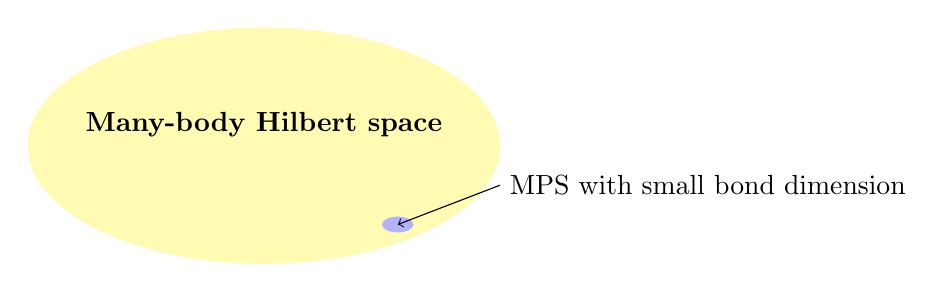
\begin{tikzpicture}
    \fill[fill=yellow!30,line width=0] (0,0) ellipse (3cm and 1.5cm) node[anchor=south] {\textbf{Many-body Hilbert space}};
    \coordinate (mpsstates) at (1.7, -1);
    \fill[fill=blue!30,line width=0] (mpsstates) ellipse (0.2cm and 0.1cm);
    \draw[<-] (mpsstates) -- (3,-0.5) node[anchor=west] {MPS with small bond dimension};
  \end{tikzpicture}
  \caption{\label{fig:mps.cartoon}%
    The manifold of quantum states with an efficient MPS description occupies only a tiny corner in the full Hilbert space.
  }
\end{figure*}
%%%%%%%%%%%%%%%%%%%%%%%%%%%%%%%%%%%%%%%%%%%%%%%%%%%%%%%%%%%%%%%%%%%%%%%%%%%%%%%%

The main application of the MPS representation in quantum information and condensed matter physics is the efficient description of certain many-body states.
As the corresponding Hilbert space grows exponentially fast in the number of constituents $N$, the full description of any state in terms of its coefficients w.r.t.\ a fixed basis is only feasible for small $N$.
Fortunately, not all quantum states of a many-body system are equally relevant in practice.
Many systems of interest are well described by a Hamiltonian with local interactions, e.g.\ nearest neighbour interactions, which reflects in the structure of correlations in their low energy spectrum.
More specifically, low energy eigenstates of gapped Hamiltonians with local interactions obey the \emph{area-law} for entanglement entropy~\cite{Hastings_2006_Solving,Verstraete_2006_Matrix,Eisert_2010_Colloquium}:
For those states, the entanglement entropy of a subsystem asymptotically only depends on its boundary size and not on its volume.
Although those stats occupy only a small corner of the enormous many-body Hilbert space as depicted in \cref{fig:mps.cartoon}, they are exceptionally important in practice.
%   - time evolution stays there -> see Orus 3.4

In one dimensional systems, any many-body state $\ket{psi}$ with an area law\footnote{%
  In one dimension, the boundary area of any connected region is constant and independent of the size of the region, and therefore, the area law implies constant entanglement entropy.
}
also has an efficient representation.
If we expand $\ket{\psi}$ in a product basis with coefficient tensor $C$,
\[
  \ket\psi = \sum_{i_1,\ldots,i_N} C_{i_1,\ldots,i_N} \, \ket{i_1} \otimes \cdots \otimes \ket{i_N},
  \label{eq:mps.state_parametrization}
\]
then $C$ can be efficiently approximated by an MPS with bond dimension scaling polynomially in $N$ and the inverse approximation error~\cite{Hastings_2006_Solving,Verstraete_2006_Matrix,Eisert_2010_Colloquium,Arad_2013_Area,Arad_2016_Rigorous}.
States of the form~\eqref{eq:mps.state_parametrization} are appropriately referred to as matrix product states.
% explains DMRG, TEBD

For higher dimensional regular latices, one can generalize the MPS representation.
The resulting efficient tensor network representation is referred to as \emph{projected entangled pair states} (PEPS).
However, a statement analogous to the one above does not hold:
For dimensions $D > 1$, not every state satisfying an area law can be efficiently represented as a PEPS.\\


%%%%%%%%%%%%%%%%%%%%%%%%%%%%%%%%%%%%%%%%%%%%%%%%%%%%%%%%%%%%%%%%%%%%%%%%%%%%%%%%
\begin{figure*}
  \centering
  \begin{tikzpicture}
    \tensor{{N=3, S=3, tensor_name='rho', tensor_width=3, tensor_height=1,
             len_vertical_legs=.5, x=-2.5}}
    \node at (rho) {$A$};

    \node at (0,0) {\Huge $=$};

    \begin{luacode*}
      mptikz.draw_mpa(3, {N=1, S=1, tensor_name='A', tensor_width=1, tensor_height=1,
                          len_vertical_legs=.5, len_horizontal_legs=.5, x=1.5})

      for i = 1, 3 do
        t('\\node[anchor=west] at (rho_N%i) {$i_%i$};', i, i)
        t('\\node[anchor=west] at (A_%i_N1) {$i_%i$};', i, i)
        t('\\node[anchor=west] at (rho_S%i) {$j_%i$};', i, i)
        t('\\node[anchor=west] at (A_%i_S1) {$j_%i$};', i, i)
        t('\\node at (A_%i) {$M\\ind{%i}$};', i, i)
      end
    \end{luacode*}

    \draw[pointerline] (A_1_N1e) -- +(0.2,0.5) node[pointernode] {row leg};
    \draw[pointerline] (A_1_S1e) -- +(0.2,-0.5) node[pointernode] {column leg};
    \draw[pointerline] (A_2_E1e) -- +(0.3,1.5) node[pointernode] {virtual leg};
  \end{tikzpicture}
  \caption{%
    \label{fig:mps.mpo}
    An MPO with open boundary condition as described.
  }
\end{figure*}
%%%%%%%%%%%%%%%%%%%%%%%%%%%%%%%%%%%%%%%%%%%%%%%%%%%%%%%%%%%%%%%%%%%%%%%%%%%%%%%%


So far, we were only concerned with multi-body pure states.
The MPS tensor format from \cref{sub:tensors.mps} can also be adapted for the description of mixed sates.
As an example consider a MPS\footnote{%
  From now on we do not distinguish between the state and its corresponding coordinate representation w.r.t.\ a fixed product basis.
}
$\ket\psi$.
The corresponding projector can be written as
\[
  \ket{\psi}\bra{\psi} =
  \begin{tikzpicture}[baseline=-.5ex]
    \mpa{4}{{N=1, y=.3, tensor_width=0.5, tensor_height=0.5, len_horizontal_legs=0.1}}
    \mpa{4}{{S=1, y=-.3, tensor_width=0.5, tensor_height=0.5, len_horizontal_legs=0.1}}
  \end{tikzpicture} =:
  \begin{tikzpicture}[baseline=-.5ex]
    \mpa{4}{{N=1, S=1, tensor_width=0.5, tensor_height=0.5, len_horizontal_legs=0.1}}
  \end{tikzpicture}
  \label{eq:mps.pure_state_projector}
\]
Here, the right hand side is a \emph{matrix product operator} (MPO).
Its local tensors $A\ind{l}$ are defined in terms of the local tensors $B\ind{l}$ of $\ket\psi$ as follows
\[
  \begin{tikzpicture}[baseline=-.5ex]
    \tensor{{N=1, S=1, W=1, E=1, tensor_name='A'}}
    \node at (A) {$A\ind{l}$};
  \end{tikzpicture}
  =
  \begin{tikzpicture}[baseline=-.5ex]
    \tensor{{N=1, W=1, E=1, tensor_name='Bu', y=0.5}}
    \node at (Bu) {$\cc{B\ind{l}}$};
    \tensor{{S=1, W=1, E=1, tensor_name='Bu', y=-0.5}}
    \node at (Bu) {${B\ind{l}}$};
  \end{tikzpicture}
  \label{eq:mps.mpdo_local_tensors}
\]
with implicit grouping of the virtual indices of $B\ind{l}$.
This is an example of a matrix-product density operator (MPDO), which were introduced in \cite{Verstraete_2004_Matrix,Zwolak_2004_MixedState}.
In general, any operator acting on the many-body Hilbert space can be expressed as an MPO with local tensors $A\ind{l} \in \Complex^{d \times d \times r \times r}$ as depicted in \cref{fig:mps.mpo}.
This representation is efficient if the operator acts \quotes{locally}, e.g.\ for a Hamiltonian with nearest neighbor interactions.

The explicit parametrization~\eqref{eq:mps.mpdo_local_tensors} of the local tensors makes it easy to see that the corresponding MPO is positive semidefinite (psd), and hence, represents a valid physical state.
A crucial question for numerical computations with density operators expressed as MPO is if there is an efficient algorithm that decides whether the
MPO is psd or not.
Unfortunately, this problem is $\NP$-hard, even if we restrict to dimensions $d=2$ and translational invariant states~\cite{Kliesch_2014_Matrix}.

%%%%%%%%%%%%%%%%%%%%%%%%%%%%%%%%%%%%%%%%%%%%%%%%%%%%%%%%%%%%%%%%%%%%%%%%%%%%%%%%
\begin{figure*}
  \centering
  \begin{tikzpicture}
    \tensor{{S=6, tensor_name='psi', tensor_width=4, tensor_height=1,
             len_vertical_legs=.5, x=-3}}
             \node at (psi) {$\ket{\psi}$};

    \node at (0,0) {\Huge $=$};

    \begin{luacode*}
      mptikz.draw_mpa(3, {S=2, tensor_name='A', tensor_width=1.5, tensor_height=1,
                          len_vertical_legs=.5, len_horizontal_legs=.25, x=2})

      for i = 1, 3 do
        t('\\node[anchor=west] at (psi_S%i) {$i_%i$};', 2 * i - 1, i)
        t('\\node[anchor=west] at (A_%i_S1) {$i_%i$};', i, i)
        t('\\node[anchor=west] at (psi_S%i) {$j_%i$};', 2 * i, i)
        t('\\node[anchor=west] at (A_%i_S2) {$j_%i$};', i, i)
      end
    \end{luacode*}

    \draw[pointerline] (A_1_S1e) -- +(-0.2,-0.5) node[pointernode,anchor=east] {physical leg};
    \draw[pointerline] (A_1_S2e) -- +(0.2,-0.5) node[pointernode] {auxilliary leg };
  \end{tikzpicture}
  \caption{%
    \label{fig:mps.pmps}
    An PMPS with open boundary condition as described.
  }
\end{figure*}
%%%%%%%%%%%%%%%%%%%%%%%%%%%%%%%%%%%%%%%%%%%%%%%%%%%%%%%%%%%%%%%%%%%%%%%%%%%%%%%%
One way to cope with this problem is to use an inherently psd parameterization of the mixed state.
Denote by $\mathcal{H}_1$ the Hilbert space of the system and by $\rho$ the corresponding mixed state.
By introducing a second \emph{auxiliary} Hilbert space $\mathcal{H}_2$, we can write~\cite{Nielsen_2010_Quantum}
\[
  \rho = \tr_{\mathcal{H}_2} \ket{\psi}\bra{\psi},
  \label{eq:mps.purification}
\]
where $\ket{\psi} \in \mathcal{H}_1 \otimes \mathcal{H}_2$.
Note that we can take $\mathcal{H}_2$ to be of the same dimension as $\mathcal{H}_1$.

Similarly, a \emph{local purification matrix product state} (PMPS)~\cite{Cuevas_2013_Purifications} is a matrix product state with two legs per site as depicted in \cref{fig:mps.pmps} such that
\[
  \underbrace{%
    \begin{tikzpicture}[baseline=-.5ex]
      \mpa{4}{{N=1, S=1, tensor_width=0.5, tensor_height=0.5, len_horizontal_legs=0.1}}
    \end{tikzpicture}
  }_{\rho}
  =
  \begin{tikzpicture}[baseline=-.5ex]
    \mpa{4}{{N=2, y=.3, tensor_width=0.5, tensor_height=0.5, len_horizontal_legs=0.1, tensor_name='up'}}
    \mpa{4}{{S=2, y=-.3, tensor_width=0.5, tensor_height=0.5, len_horizontal_legs=0.1, tensor_name='down'}}
    \draw[tensorleg] (up_1_N2e) to[out=75,in=-75] (down_1_S2e);
    \draw[tensorleg] (up_2_N2e) to[out=75,in=-75] (down_2_S2e);
    \draw[tensorleg] (up_3_N2e) to[out=75,in=-75] (down_3_S2e);
    \draw[tensorleg] (up_4_N2e) to[out=75,in=-75] (down_4_S2e);
  \end{tikzpicture}
  \label{eq:mps.pmps}
\]
This is an inherently positive semidefinite parametrization of $\rho$ in matrix product form.
However, this advantage comes at a price:
The PMPS representation of a state can be arbitrarily more costly than its MPDO representation~\cite{Cuevas_2013_Purifications}.
More precisely, there a families of states $(\rho_N)_{N \in \Naturals}$  with $\rho_N \in \Complex^{d^N}$ such that $\rho_N$ has constant MPO-rank, but the PMPS-rank of $rho_N$ scales as $\Order(N)$.
This and the hardness result from~\cite{Kliesch_2014_Matrix} shows that no efficient algorithm for computing an exact local purification from an MPDO exists in general.
However, the questions how generic this hardness is and how hard approximative versions of this problem are remain open?\\



Besides the original applications in physics, the MPS tensor format has recently also found applications in the field of machine learning:
Deploying the latest neural networks on mobile devices such as smart phones or IOT devices is challenging due to the high dimensional hidden layers, e.g. a single weight matrix of a fully connected layer can have millions of parameters.
By approximating this weight matrix by an MPS with small bond dimension, the authors in~\cite{Novikov_2015_Tensorizing} were able to compress state-of-art image detection networks by a factor of seven with only minor performance penalties.
Other examples of applications of tensor decompositions in deep learning include regularization~\cite{Tai_2015_Convolutional} and deep representation learning~\cite{Yang_2016_Deep}.

Another use of the MPS tensor format in machine learning was pioneered in~\cite{Stoudenmire_2016_Supervised}.
They consider a support vector machine classifier, which for the binary (yes/no) outcome is given by
\[
  f(X) = \braket{W, X},
\]
where $X$ is the input vector and $W$ is the model vector.
The goal is to determine $W$ in such a way that $f(X) > 0$ if $X$ is in the \quotes{yes} class and $f(X) < 0$ otherwise.
By using a MPS representation for $W$ and $X$, they are able to efficiently learn such a model even in high-dimensional settings.
A similar can also be applied to learning polynomial classifiers~\cite{Chen_2017_Parallelized} as well as for image compression and classification~\cite{Bengua}.



%%%%%%%%%%%%%%%%%%%%%%%%%%%%%%%%%%%%%%%%%%%%%%%%%%%%%%%%%%%%%%%%%%%%%%%%%%%%%%%%
\section{The Python Library mpnum}%
\label{sec:tensors.mpnum}

\input{notebooks/Introduction}
\todo{Examples for thermal state computation}


%%%%%%%%%%%%%%%%%%%%%%%%%%%%%%%%%%%%%%%%%%%%%%%%%%%%%%%%%%%%%%%%%%%%%%%%%%%%%%%%
\section{Scalable maximum likelihood estimation for quantum states}%
\label{sec:tensors.mle}

\todo{Leave this out?}
% QSE -> see chapter ..., number of measurements without further assumptions ~ dimension of hilber space ^2 -> exponential for many body states
% slight reduction using low-rank matrix recovery, but still exponential
% here: assuming efficient MPO description -> # of measurements -> linear in N
%

%%%%%%%%%%%%%%%%%%%%%%%%%%%%%%%%%%%%%%%%%%%%%%%%%%%%%%%%%%%%%%%%%%%%%%%%%%%%%%%%
\section{Efficient low-rank tensor reconstruction}%
\label{sec:tensors.als}

%%%%%%%%%%%%%%%%%%%%%%%%%%%%%%%%%%%%%%%%%%%%%%%%%%%%%%%%%%%%%%%%%%%%%%%%%%%%%%%%
\begin{figure*}
  \centering
  \begin{tikzpicture}
  \mpa{6}{{tensor_height=1, tensor_width=1, virtual=0, len_horizontal_legs=.5,
           tensor_style='rounded corners=.5cm, fill=black!40'}}
  \node[below= 0 of X_2] () {$\sigma\ind{1}_{i_1}$};
  \node[below= 0 of X_3] () {$\sigma\ind{2}_{2_1}$};
  \node[below= 0 of X_4] () {$\sigma\ind{3}_{3_1}$};

  \begin{scope}[on background layer]
	\fill[fill=blue!10, rounded corners=.1cm] ($ (X_2) - (0.75,1.75) $) rectangle ($ (X_4) + (0.75,0.75) $);
  \end{scope}
  \draw [thick, decoration={brace}, decorate] ([yshift=1cm]X_1.west) -- node[above=3mm] {$N$} ([yshift=1cm]X_6.east);
  \draw [thick, decoration={brace, mirror}, decorate] ([yshift=-2cm]X_2.west) -- node[below=3mm] {$R$} ([yshift=-2cm]X_4.east);

\end{tikzpicture}

  \caption{%
    The local measurements used for the reconstruction of MPS, MPO, and unitary channels in~\cite{Cramer_2010_Efficient,Baumgratz_2013_Scalable,Baumgratz_2013_Scalablea,Lanyon_2017_Efficient,Holzaepfel_2014_Scalable}.
    These consist of informationally complete measurements on blocks of $R$ consecutive qudits, e.g.\ all Pauli product measurements on $R$ qudits.
    }%
  \label{fig:als.quantum_measurements}
\end{figure*}
%%%%%%%%%%%%%%%%%%%%%%%%%%%%%%%%%%%%%%%%%%%%%%%%%%%%%%%%%%%%%%%%%%%%%%%%%%%%%%%%

With the ability to approximate structured tensors from many applications efficiently in MPS form, one crucial question remains:
How can we \emph{efficiently} recover this representation in practice from measurable quantities?
Here, \quotes{efficiency} refers to two different aspects.
On the one hand, we want to bound the number of measurements required to perform reconstruction, i.e.\ the \emph{sample complexity}.
On the other hand, it refers to the \quotes{computational complexity} as outlined in \cref{sec:error.complexity}
Both aspects are especially critical for tensor reconstruction as na\"ive approaches generally suffer from the curse of dimensionality.

In the context of quantum estimation, existing work addresses this question for the reconstruction of MPS~\cite{Cramer_2010_Efficient}, MPDO~\cite{Baumgratz_2013_Scalable,Baumgratz_2013_Scalablea,Lanyon_2017_Efficient}, and unitary quantum processes~\cite{Holzaepfel_2014_Scalable} from local measurements.
More precisely, they consider measurements that act non-trivially only on blocks of $R$ adjacent qudits as depicted in \cref{fig:als.quantum_measurements}.
This results in a sample complexity scaling as $\Order(N \times d^R)$ compared to the $m = \Order(d^N)$ for the na\"ive approach.
Numerical experiments in~\cite{Cramer_2010_Efficient,Baumgratz_2013_Scalable,Baumgratz_2013_Scalablea} demonstrate successful recovery of W-states as well as ground and thermal states of nearest-neighbor Hamiltonians for small values of $R$ independent of $N$.
Naturally, these are all examples of MPS or MPO with small bond dimension.
The drastically reduced sampling complexity makes the approaches efficient and viable for large-scale quantum experiments.
However, only the numerically inferior algorithm\footnote{%
  T.\ Baumgratz, private communications.
}
from~\cite{Baumgratz_2013_Scalable} comes with a proof of convergence.
Similar rigorous recovery guarantees have only been proven for comparable, but inefficient versions of the algorithms in~\cite{Cramer_2010_Efficient,Baumgratz_2013_Scalablea}.\\



The question that motivated the work presented in this chapter is whether we can identify other measurement schemes and algorithms that \emph{provably} allow for efficiently reconstructing low-rank tensors.
Recall that we already encountered a similar question in \cref{cha:phaselift} for the problem of \emph{low-rank matrix recovery}.
The latter asks under which conditions we can recover a low-rank matrix $X \in \Complex^{d \times d}$ from $m$ linear measurements of the form
\[
  y\ind{l} = \braket{A\ind{l}, X}, \quad l=1, \ldots, m.
  \label{eq:als.matrix_measurements}
\]
Here, $A\ind{l} \in \Complex^{d \times d}$ denote the measurement matrices and
\[
  \braket{A, X} = \tr \adj{A} X
\]
the Frobenius inner product.
For a general matrix $X$, the number of measurements $m$ needs to scale as $d^2$ by the pigeonhole principle.
However, by exploiting the low-rank structure of $X$, we can reduce $m$.
For example, \cref{thm:???} shows that we can recover any positive semi-definite rank-1 matrix $X$ from only $m = \Order(d)$ measurements provided the $A\ind{l}$ are sampled from an appropriate distribution of random matrices.
Furthermore, said theorem also provides an efficient reconstruction algorithm, namely the semi-definite program~\eqref{eq:???}.

More generally, we can recover any $X \in \Complex^{d \times d}$ with $\rank X = r$ from $m = \Order(d r)$ randomly chosen measurements~\cite{Candes_2011_Tight,Kueng_2014_Low}.
Intuitively, this sample complexity is asymptotically optimal since we need at least $2 d r$ complex parameters to specify the left- and right-singular vectors of $X$, see~\cite{Eldar_2012_Uniqueness,Li_2017_Optimal} for rigorous lower bounds.\\




Here, we consider the generalization of low-rank matrix recovery to higher order tensors\footnote{%
  In contrast to the rest of this chapter, we consider real tensors in order to simplify notation.
}
$X \in \Reals^{d^N}$ of low MPS-rank.
For this purpose, we study an \emph{Alternating Least Squares} (ALS) algorithm inspired by DMRG methods in quantum physics.
The observable quantities are -- analogous to \cref{eq:als.marix_measurements} -- given by overlaps with measurement tensors $A\ind{l} \in \Reals$
\[
  y\ind{l} = \braket{A\ind{l}, X}
  \label{eq:als.tensor_measurements}
\]
with the Frobenius inner product of tensors defined by \cref{eq:mps.inner}.

The field of low-rank tensor recovery has attracted increasing attention in recent years.
Especially the problem of tensor completion, i.e.\ inferring missing values of a low-rank tensor, has been thoroughly studied due to its broad applicability in computer vision, neuroscience, remote sensing, and context-aware recommender systems~\cite{Li_2010_Tensor,Zhu_2016_ContextAware,Wang_2014_LowRank}.
In contrast to our work, most analytical results in this area are concerned with different notions of tensor rank such as the Tucker rank~\cite{Kressner_2013_LowRank,Zhang_2016_Cross} or the canonical tensor rank~\cite{Krishnamurthy_2013_LowRank,Potechin_2017_Exact}.
\todo{Why Tucker/canonical bad?, Why TT good}

The best analytical recovery guarantees for low-MPS rank tensor completion require -- to the best of the authors knowledge -- a number of measurements scaling exponentially in the order of the tensor~\cite{Phien_2016_Efficient}.
Although their result gives a square-root advantage compared to na\"ive reconstruction, it is still infeasible for high-order tensors.
However, numerical investigations using an alternating least squares algorithm similar to the one used in this work demonstrate successful recovery with sub-exponential sample complexity~\cite{Grasedyck_2015_Variants,Wang_2016_Tensor}.

% low-rank approximation
% Riemannian optimization -> Lubich
% ALtmin local convergence for Optimization-> Rohwedder, Uschmajew; Holtz, Rohwedder\tabularnewline

Stronger analytical results exist for a different measurement ensemble:
The authors in~\cite{Rauhut_2014_Tensor}, consider fully Gaussian measurements, i.e.\ measurement tensors with independent components sampled from a normal distribution.
In this approach, a number of such measurements scaling polynomially in the crucial parameters $d$, $N$, and $r$ is sufficient to recover any rank $r$ tensor.
Although their result is highly sample efficient, it is still infeasible for high-order tensors due to the exponentially scaling memory requirement for the measurement tensors.

In conclusion, the existing rigorous work on recovering low MPS-rank tensors is currently situated at two different ends of a spectrum:
On the on hand, there is tensor completion, which is highly relevant for practical applications and efficiently implementable, but without any recovery guarantees for a polynomially scaling number of measurements.
On the other hand, the authors in~\cite{Rauhut_2014_Tensor} prove reconstruction with near-optimal sample complexity, but their full Gaussian measurements are computationally very demanding.

This situation can be understood better by comparing to the history of low-rank matrix recovery and compressive sensing -- the related problem of reconstructing sparse vectors from few measurements.
The first rigorous on compressed sensing from Gaussian measurements were due to Donoho~\cite{For_most} in 2006.
In the same year, Candes and Tao -- a Fields medalist -- proved guarantees for orthonormal basis vector measurements~\cite{Stable_signal}, which can be considered as the analogue of matrix completion for vectors.
The same authors also proved the first matrix recovery guarantees for Gaussian sampling matrices~\cite{} and for matrix completion~\cite{}.
Here, we are going to study a measurement ensemble for tensors that combines the advantages of both approaches.
We take the measurement tensors to be of the form
\[
  A\ind{l} = a\ind{l}_1 \otimes \cdots a\ind{l}_N
  \label{eq:als.rank1_measurements}
\]
with local tensors randomly chosen from a standard multivariate normal distribution $a\ind{l}_k \sim \Normal(0, \1_d)$.
In contrast to the fully Gaussian model from~\cite{}, the measurement tensors~\eqref{eq:als.rank1_measurements} can be represented efficiently as MPS of unit rank.
And, unlike the tensor completion problem, history does not dictate that its solution requires at least one Fields medalist.



\subsection{The alternating least squares algorithm}%

In this section, we are going to report on work in progress for the problem of reconstructing low-rank tensors from few measurements.
To recapitulate, the goal is to recover a tensor $X \in \Reals^{d^N}$ with MPS-rank\footnote{%
  From now on, we simply say \quotes{rank} instead of \quotes{MPS-rank}.
} $r$ from $M$ linear measurements of the form
\[
  b\ind{l} = \braket{A\ind{l}, X}, \ldots l=1,\ldots,M,
\]
where $A\ind{l}$ is a product of Gaussian vectors as defined in \cref{eq:als_rank1_measurements}.
For this purpose, we want an efficient reconstruction algorithm and $m$ to scale polynomially in the parameters $d$, $N$, and $r$.

The idea to recover $X$ is simply to find the tensor $Y$ of desired rank that minimizes the empirical $\ell_2$ error
\[
  \sum_l \left( y\ind{l} - \braket{A\ind{l}, Y} \right)^2.
  \label{eq:als.empirical_l2}
\]
However, this problem is generally hard to solve directly since the space of MPS of given rank is non-convex.
Nevertheless, in the case of $M=\Order(???)$ fully Gaussian measurements, a projected gradient descent on~\eqref{eq:als.empirical_l2} is able to recover $X$.
However, the same proof techniques fail in the case of structured measurements such as the ones defined in \cref{eq:als.rank1_measurements} as we show in \cref{???}.

Instead of updating each local tensor at the same time as in the gradient descent, we iteratively optimize the empirical error over a single local tensor at a time.
The resulting algorithm is presented below:

\begin{algorithm}[H]
  \caption{\label{alg:als}Alternating Least Squares (ALS) for $\ell_2$ minimization}
  \SetKwInOut{Input}{Input}
  \SetKwInOut{Output}{Output}

  \Input{%
    Measurement tensors $A\ind{l}$, measurement outcomes $y\ind{l}$, target rank $r$, and number of epochs $H$ \newline
    Divide $(A\ind{l}, y\ind{l})_l$ into $HN + 1$ subsets of size $m$, which are denoted by ${\left(A\ind{0;l}, y\ind{0;l}\right)}_l$ and ${\left(A\ind{h,n;l}, y\ind{h,n;l}\right)}_l$ ($h \in [H], n \in [N]$)
  }
  \BlankLine

  \tcc{Initialize $Y$ as MPS with given rank}
  $Y \gets \mathtt{compress}\left(\sum_{l=1}^m y\ind{0;l} A\ind{0;l}, r\right)$ \label{line:als.initialization}

  \For{$h \gets 1$ \KwTo $H$}{
    \tcc{right-normalize all local tensors}
    $\mathtt{right\-canonicalize}(Y)$ \label{line:als.right_canonical}

    \For{$n \gets 1$ \KwTo $N$}{
      \For{$l \gets 1$ \KwTo $m$} {
        \tcc{contract $A\ind{h,n;l}$ with all but n-th local tensors of $X$}
        $B\ind{l} \gets \mathtt{contract}(A\ind{h,n;l}, X_{[N] \backslash n})$ \label{line:als.partial_contraction}
      }
      $\hat Z \gets \argmin_Z \sum_l \left( y\ind{h,n;l} - B\ind{l}Z   \right)^2$ \label{line:als.min}

      \tcc{update the n-th local tensor inplace}
      $Y_n \gets \mathtt{left\_normalize}(\hat Z)$
    }
  }

  \Output{Y}
\end{algorithm}
\todo{Update initialization?}

In this version of the alternating least squares scheme, we start updating the left-most tensor and then move through the chain all the way to the right.
When we reach the last tensor of the MPS, we start again on the left after bringing the MPS to right-canonical form.
Hence, all tensors to the left and right of the currently updated tensor are left- and right-normalized, respectively.
This process is repeated $H$ number of times.
In practice, we make the algorithm slightly faster by skipping the right-canonicalization step in line~\ref{line:als.right_canonical} and perform a sweep left-right-left instead.

The crucial step in this algorithm is the local minimization in line~\ref{line:als.min}.
It amounts to keeping all but the $n$-th local tensor of $Y$ fixes and minimizing the empirical error over $Y_n$.
The minimizer $\hat Z$ can be computed efficiently from the linear least squares problem
\[
  \hat Z
  = \argmin_Z \sum_l \left( y\ind{h,n;l} - B\ind{l}Z   \right)^2
  = \norm{y\ind{h,n} - B Z}_{\ell_2}^2.
  \label{eq:als.llsq}
\]
Here, the rows of the matrix\footnote{%
  More precisely, we have $B \in \Reals^{m \times (rd)}$ for $n=1$ or $n=N$.
}
$B \in \Reals^{m \times (dr^2)}$ are defined in line~\ref{line:als.partial_contraction} in terms of partial contractions of $A\ind{h,n;l}$ and $Y$ leaving out the $n$-th local tensor of $Y$:
\[
  B\ind{l} =
  \begin{tikzpicture}[baseline=-.5ex]
    \mpa{{1,2,4,5,6}}{{S=1, y=.5, tensor_height=0.5, tensor_width=0.5, tensor_name='Y'}}
    \mpa{6}{{N=1, virtual=0, y=-.5, tensor_height=0.5, tensor_width=0.5, tensor_name='A'}}

    \draw[pointerline] (Y_6) -- +(1,.125) node[pointernode] {$Y$};
    \draw[pointerline] (A_6) -- +(1,-.125) node[pointernode] {$A\ind{h,n;l}$};
  \end{tikzpicture}
  \label{eq:als.minimization_matrix}
\]
Therefore, the solution $\hat Z$ of \cref{eq:als.llsq} is a $d r^2$ dimensional vector, which can be reshaped to the correct form.
If we replace the exact local minimization in \cref{eq:als.llsq} by a finite gradient descent step, we obtain a standard nonlinear block Gauss–Seidel iteration~\cite{Schechter}.

Finally, note that the sample splitting at the beginning is necessary for the analysis of the algorithm below as it requires independent updates at each step.
Therefore, we use a fresh batch of measurement tensors and measurement values in each step, which results in a total number of $M = (HN + 1)m$ measurements.
Provided that both $H$ and $m$ scale polynomially in the system's parameters, then so does $M$.
However, numerical experiments below show that this resampling is unnecessary in practice.\\



Alternating algorithms such as ALS updating only a few local tensors at a time are a very common approximation technique for circumventing intractabilities when dealing with MPS.
Well known examples include variational compression and DMRG~\cite{Schollwoeck} --  an iterative algorithm for approximating the smallest eigenvalue of a hermitian MPO.
Local convergence of these alternating algorithms has been proved for a large class of problems in~\cite{Rohwedder}.
However, these result only show that the ALS algorithm converges to a local minimum, which unless the initialization is chosen well differs from the target tensor $X$.
Furthermore, it remains to be shown that the minimizer of the empirical $\ell_2$ error~\eqref{eq:als.empirical_l2} with given rank is equal to $X$, i.e.\ that the given measurements suffice to identify $X$.


\subsection{Analysis of the ALS}%
\label{sub:als.ana}

We now turn to the problem of analysing \cref{alg:als}, generalizing the ideas from~\cite{Zhong} to the tensor case.
For the sake of simplicity, we are only going to treat the case of a product signal tensor, i.e.\ $X$ is assumed to have rank one.
Furthermore, we also assume w.l.o.g.\ that $X$ is normalized in Frobenius norm, i.e.\ $\norm{X}_2 = 1$.
Then, $X$ can be written as a tensor product of $N$ normalized vectors $x_i \in \Reals^d$ and we have
\[
  b\ind{l} = \braket{A\ind{l}, X} = \prod_{i=1}^N \braket{a\ind{l}_i, x_i}.
  \label{eq:ana.b_as_product}
\]
One main result of this chapter is \cref{thm:ana.local_convergence}.
It shows that under certain assumptions on the initialization and measurement tensors, each micro-iteration brings the local tensor closer to its true value in a suitable metric.
In the case of rank-1 tensor reconstruction, this metric between the local tensors $x$ and $y$ with $\ltwonorm{x} = \ltwonorm{y} = 1$ is given by
\[
  \mathrm{dist}(x, y) = \sqrt{1 - \Abs{\braket{x, y}}^2}.
  \label{eq:ana.infidelity}
\]
It is known as \emph{infidelity} if $x, y \in \Complex^d$ represent pure quantum states~\cite{Nielsen_2010_Quantum}.
\Cref{eq:ana.infidelity} is also the one-dimensional special case of the \emph{principle angle distance} of subspaces~\cite{Golub}, which is the appropriate distance measure for higher-rank generalizations of the results presented here.

In the first lemma, we relate the \quotes{global} distance of two tensors, which is measured in Frobenius norm, to the distances of the local tensors.
\begin{lemma}%
  \label{lem:ana.local_global_closeness}
  Let $X = \otimes_{i=1}^N x_i$ and $Y = \otimes_{i=1}^N y_i$ be two product tensors of unit norm.
  Assume that for each $i \in \Nset$, we have $\ltwonorm{x_i} = \ltwonorm{y_i} = 1$ and
  \[
    \label{eq:ana.local_global_closeness.local_close}
    1 - \Braket{x_i, y_i}^2 \le \delta_i^2.
  \]
  Then,
  \[
    \min_{\eta = \pm 1} \Fnorm{X - \eta Y} \le \sqrt{2} \sum_{i=1}^N \delta_i.
  \]
\end{lemma}
\begin{proof}
  First, note that \cref{eq:ana.local_global_closeness.local_close} implies
  \begin{align}
    \min_{\eta = \pm 1} \ltwonorm{x_i - \eta y_i}^2
    &= \min_{\eta = \pm 1} 2 (1 - \eta \braket{x_i, y_i})
    = 2 (1 - \abs{\braket{x_i, y_i}}) \\
    &\le 2 (1 - \braket{x_i, y_i}^2)
    \le 2 \delta_i^2.
  \end{align}
  Therefore, we get for the Frobenius norm distance of the full tensors
  \begin{align}
    \min_{\eta=\pm1} \Fnorm{X - \eta Y}
    &= \min_{\eta \in \{\pm1\}} \Fnorm{x_1 \otimes \cdots \otimes x_N - \eta\, y_1 \otimes \cdots y_N} \\
    &\begin{aligned}
      \le \min_{\eta,\xi \in \{\pm1\}} \Large(
        \Fnorm{x_1 \otimes x_2 \otimes \cdots \otimes x_N - \eta \xi \, x_1 \otimes y_2 \otimes \cdots \otimes y_N} \\
        + \Fnorm{\eta \xi \, x_1 \otimes y_2 \otimes \cdots \otimes y_N - \eta\, y_1 \otimes y_2 \otimes \cdots y_N}
      \Large)
    \end{aligned}\\
    &\begin{aligned}
      = \min_{\eta\in\{\pm1\}} \Fnorm{x_2 \otimes \cdots \otimes x_N - \eta \, y_2 \otimes \cdots \otimes y_N} \\
        + \min_{\eta\in\{\pm1\}} \Fnorm{x_1 - \eta\, y_1}.
    \end{aligned}
  \end{align}
  By telescoping this argument, we get
  \[
    \min_{\eta = \pm 1} \ltwonorm{x_i - \eta y_i}^2
    \le \sum_{i=1}^N \left( \min_{\eta\in\{\pm1\}} \Fnorm{x_i - \eta y_i} \right)
    \le \sqrt{2} \sum_{i=1}^N \delta_i,
  \]
  which completes the proof.
\end{proof}

We now turn to the main problem in this section, namely providing upper bounds on the ALS-reconstruction.
For this purpose, we assume that the following two conditions hold for our measurements:
\begin{enumerate}
  \item\label{lbl:conditions.B}\textbf{Concentration of the $B_j$ operators}:
    For all $j \in \Nset$, let $v_i \in \Reals^d$ with $\norm{v_i}_2 = 1$ ($i \in \NsetSub{j}$) independent of all the $a\ind{l}_i$.
    Define
    \[
      \label{eq:ana.conditions.B}
      B_j\left((v_i)_{i \in \NsetSub{j}}\right)
      = \frac{1}{m} \sum_{l=1}^m \left( \prod_{i\neq j} \Braket{a\ind{l}_i, v_i} \right)^2 \Ketbra{a_j\ind{l}},
    \]
    Then, the smallest eigenvalue of $B_j\left((v_i)_{i \in \NsetSub{j}}\right)$ should satisfy
    \[
      \label{eq:ana.conditions.lmin}
      \lambda_\mathrm{min}\left(B_j\left((v_i)_{i \in \NsetSub{j}}\right)\right) \ge \delB
    \]
    for some constant $\delB > 0$
  \item\label{lbl:conditions.G}\textbf{Concentration of the $G_j$ operators}:
    For all $j \in [N]$, let $v_i, v_i^\perp \in \Reals^d$ ($i \in \NsetSub{j})$ independent of all the $a\ind{l}_i$.
    Furthermore, they should satisfy $\norm{v_i}_2 = \norm{v_i^\perp}= 1$ and $\braket{v_i, v_i^\perp} = 0$ for $i\in\NsetSub{j}$.
    Define
    \[
      \label{eq:ana.conditions.G}
      G_j\left({(v_i, v_i^\perp)}_{i \in \NsetSub{j}} \right)
      = \frac{1}{m} \sum_{l=1}^m \left( \prod_{i\neq j} \Braket{a\ind{l}_i, v_i} \Braket{a\ind{l}_i, v_i^\perp} \right) \Ketbra{a_j\ind{l}}.
    \]
    Then, with high probability the largest singular value of $G_j\left({(v_i, v_i^\perp)}_{i \in \NsetSub{j}} \right)$ should satisfy
    \[
      \label{eq:ana.conditions.lmax}
      \Opnorm{G_j\left({(v_i, v_i^\perp)}_{i \in \NsetSub{j}} \right)} \le \delG.
    \]
    for some constant $\delG > 0$
\end{enumerate}
In \cref{sub:als.gaussian_measurements} we elaborate on work in progress with the goal of proving that random local tensors $a\ind{l}_i$ sampled independently from a standard $d$-variate Gaussian distribution satisfy these conditions with high probability.\\


We start the analysis by examining a single update step in \cref{alg:als} for the leftmost local tensor with $n = 1$.
Denote by $\tilde y^{h+1}_1$ the minimizer $\hat Z$ in line~\ref{line:als.min} and by $y^h_i$ the remaining local tensors of $Y$, which are kept fixed during this micro-iteration.
The empirical error as a function of $\tilde y^{h+1}_n$ then reads
\[
  F\left(\tilde y^{h+1}_1\right)
  = \sum_l {\left(  \prod_i \braket{a\ind{l}_i, x_i} - \braket{a\ind{l}_1, \tilde y^{h+1}_1} \, \prod_{i \neq 1} \braket{a\ind{l}, y^{h}_i} \right)}^2
  \label{eq:ana.l2_error}
\]
Since in the following, we only consider the optimization over $\tilde y^{h+1}_1$ and keep the other $y^h_i$ fixed, we write $\tilde y_1$ and $y_i$ (for $i > 1$), respectively, if there is no risk of confusion.
In contrast to the $(y_i)_{i > 1}$, $\tilde y_1$ is not normalized.
We now derive an explicit representation of the minimizer of \cref{eq:ana.l2_error}.

\begin{lemma}%
  \label{lem:ana.gradient_of_error}
  Denote by $F$ the empirical $\ell_2$ error defined in \cref{eq:ana.l2_error}.
  Then, the extremal point $\tilde y_1$ with $\frac{\partial F(\tilde y_1)}{\partial \tilde y_1} = 0$ is given by
  \[
    \Ket{\tilde y_1} = {\left( \prod_{i \neq 1} \Braket{x_i, y_i} \right)} \Ket{x_1} - \tilde B_1^{-1} \tilde G_1 \Ket{x_1}
    \label{eq:ana.gradient_of_error}
  \]
  with $\tilde B_1$ and $\tilde G_1$ given by
  \begin{align}
    \label{eq:ana.b_operator}
    \tilde B_1 &= \frac{1}{m} \sum_l {\left( \prod_{i \neq 1} \Braket{a\ind{l}_i,y_i} \right)}^2 \Ketbra{a\ind{l}_1} \\
    \label{eq:ana.g_operator}
    \tilde G_1 &= \frac{1}{m} \sum_l {\left( \prod_{i \neq 1} \Braket{a\ind{l}_i, \tilde y_i^\perp} \Braket{a\ind{l}_i,y_i} \right)}\Ketbra{a\ind{l}_1} \\
    \tilde y_i^\perp &= \left(\ketbra{y_i} - \1 \right) x_i \quad(i \in \NsetSub{1}).
  \end{align}
\end{lemma}
\begin{proof}
  We begin by computing the derivative of $F$
  \[
    \frac{\partial F(\tilde y_1)}{\partial \tilde y_1}
    = -2 \sum_l \left( \prod_i \Braket{a\ind{l}_i, x_i} - \Braket{a\ind{l}_1, \tilde y_1} \, \prod_{i \neq 1} \Braket{a\ind{l}_i, y_i} \right) \, \left( \prod_{i \neq 1} \Braket{a\ind{l}_i, y_i} \right) \, \Ket{a\ind{l}_1},
  \]
  which is equal to zero if and only if
  \[
  \sum_l \left( \Braket{a\ind{l}_1, \tilde y_1} \, \prod_{i \neq 1} \Braket{a\ind{l}_i, y_i} \prod_{i \neq 1} \Braket{a\ind{l}_i, y_i} \right) \, \Ket{a\ind{l}_1}
  =
  \sum_l \left( \prod_i \Braket{a\ind{l}_i, x_i} \prod_{i \neq 1} \Braket{a\ind{l}_i, y_i} \right) \, \Ket{a\ind{l}_1}.
  \]
  Reordering terms and factoring out the terms with $i = 1$ gives
  \[
  \sum_l {\left(\prod_{i \neq 1} \Braket{a\ind{l}_i, y_i} \right)}^2 \, \Ket{a\ind{l}_1} \Braket{a\ind{l}_1, \tilde y_1}
  =
  \sum_l \left( \prod_{i \neq 1} \Braket{a\ind{l}_i, x_i} \Braket{a\ind{l}_i, y_i} \right) \, \Ket{a\ind{l}_1} \Braket{a\ind{l}_1, x_1},
  \]
  and therefore,
  \[
    \tilde  B_1 \Ket{\tilde y_1} =
    \underbrace{ \frac{1}{m} \left[ \sum_l \left( \prod_{i \neq 1} \Braket{a\ind{l}_i, x_i} \Braket{a\ind{l}_i, y_i} \right) \, \Ketbra{a\ind{l}_1} \right]}_{=: \tilde O_1} \Ket{x_1}.
  \]
  Note that $\tilde B_1 = B_1(y_2, \ldots, y_N)$ as defined in \cref{eq:ana.conditions.B}.
  Since we assume by \cref{eq:ana.conditions.lmin} that the smallest eigenvalue of $\tilde B_1$ is larger than zero, it is invertible and we can multiply the last equation by its inverse and obtain
  \[
    \Ket{\tilde y_1} = \left( \prod_{i \neq 1} \Braket{x_i, y_i} \right) \Ket{x_i} - \tilde B_1^{-1} \left( \left(\prod_{i \neq 1} \Braket{x_i, y_i} \right) \tilde B_1 - \tilde O_1 \right) \Ket{x_i},
  \]
  where the first and second summand cancel each other.
  Finally, we simplify the expression in parentheses, which completes the proof:
  \todo{Fix alignment}
  \begin{flalign}
    \left(\prod_{i \neq 1} \Braket{x_i, y_i} \right) \tilde B_1 - \tilde O_1 \\
    &= \frac{1}{m} \sum_l \left( \prod_{i \neq 1} \braket{x_i, y_i}\braket{a\ind{l}_i, y_i}^2 - \prod_{i \neq 1} \braket{a\ind{l}_i, y_i}\braket{a\ind{l}_i, x_i} \right) \Ketbra{a\ind{l}_1} \\
    &= \frac{1}{m} \sum_l \left( \prod_{i \neq 1} \braket{a\ind{l}_i, y_i} \left(\braket{x_i, y_i}\braket{a\ind{l}_i, y_i} - \braket{a\ind{l}_i, x_i} \right) \right) \Ketbra{a\ind{l}_1} \\
    &= \frac{1}{m} \sum_l \left( \prod_{i \neq 1} \braket{a\ind{l}_i, y_i} \left(\Braket{a\ind{l}_i, \braket{y_i, x_i} y_i - x_i} \right) \right) \Ketbra{a\ind{l}_1} \\
    &= \tilde G_1.
  \end{flalign}
\end{proof}

From \cref{eq:ana.gradient_of_error} we see that if the error term $\tilde B_1^{-1} \tilde G_1 \ket{x_1}$ is small, then the overlaps of the remaining local tensors $\braket{x_i, y_i}$ for $i=2,\ldots,N$ determine how close $\tilde y_1$ is to its true value $x_1$.
The following lemma makes this precise.

\begin{lemma}%
  \label{lem:ana.local_error_bound}
  Let $\ket{y_1} := \frac{\ket{\tilde y_1}}{\ltwonorm{\tilde y_1}}$ with $\ket{\tilde y_1}$ given by \cref{eq:ana.gradient_of_error}.
  Furthermore, define
  \[
    \label{eq:ana.local_error_bound.def_kappa}
    \kappa_1 = \frac{\delB}{\delG} \prod_{i \neq 1} \Abs{\braket{x_i, y_i}} - \prod_{i \neq 1} \sqrt{1 - \braket{x_i, y_i}^2}.
  \]
  Assume that the conditions of \cref{eq:ana.conditions.lmin,eq:ana.conditions.lmax} hold and $\kappa_1 > 0$, then we have
  \[
    \label{eq:ana.local_error_bound}
    1 - \Braket{x_1, y_1}^2 \le \frac{\prod_{i \neq 1} (1 - \braket{x_i, y_i}^2)}{\kappa_1^2}.
  \]
\end{lemma}
\begin{proof}
  First recall that $\tilde B_1 = B_1(y_2, \ldots, y_N)$ as defined in \cref{thm:ana.conditions.B}.
  Since $\ltwonorm{y_i} = 1$ and $\tilde B_1$ is positive definite, the lower bound on the smallest eigenvalue of $\tilde B_1$ in \cref{eq:ana.conditions.lmin} translates to
  \[
    \label{eq:ana.error_term_bound.B}
    \Opnorm{\tilde B_1^{-1}} = \frac{1}{\lambda_\mathrm{min}(\tilde B_1)} \le \frac{1}{\delB}.
  \]
  Furthermore, $\tilde G_1 = G_1(y_2, \tilde y_2^\perp, \ldots, y_N, \tilde y_N^\perp)$, and hence, normalization of the $\tilde y_i^\perp$ yields
  \[
    \label{eq:ana.error_term_bound.G}
    \begin{split}
      \Opnorm{\tilde G_1}
      &\le \delG \prod_{i \neq 1} \ltwonorm{\tilde y_i^\perp} \\
      &\le \delG \prod_{i \neq 1} \sqrt{1 - {\braket{x_i, y_i}}^2}.
    \end{split}
  \]
  Combining \cref{eq:ana.error_term_bound.B,eq:ana.error_term_bound.G} as well as the condition $\ltwonorm{x_1} = 1$ yields the bound on the error term
  \[
    \label{eq:ana.error_term_bound}
    \Ltwonorm{\tilde B_1^{-1} \tilde G_1 x_1}
    \leq \frac{\delG}{\delB} \, \prod_{i \neq 1} \sqrt{1 - {\braket{x_i, y_i}}^2}.
  \]
  Next, using \cref{eq:ana.gradient_of_error}, we can lower bound the overlap
  \begin{align}
    \Abs{\braket{x_1, \tilde y_1}}
    &= \Abs{\prod_{i \neq 1} \braket{x_i, y_i} - \braket{x_i, B_1^{-1} G_1 x_1}} \\
    &\ge \Abs{\prod_{i \neq 1} \abs{\braket{x_i, y_i}} - \Abs{\braket{x_1, B_1^{-1} G_1 x_1}}} \\
    &\ge {\prod_{i \neq 1} \Abs{\braket{x_i, y_i}} - \Ltwonorm{B_1^{-1} G_1 x_1}} \\
    &\ge {\prod_{i \neq 1} \Abs{\braket{x_i, y_i}} - \frac{\delG}{\delB} \prod_{i \neq 1} \sqrt{1 - {\braket{x_i, y_i}}^2}}.
    \label{eq:ana.local_error_bound_step.overlap_x}
  \end{align}
  by the Cauchy-Schwartz inequality and \cref{eq:ana.error_term_bound}.
  Along the same lines, we obtain for any $x_1^\perp$ with $\ltwonorm{x_1^\perp} = 1$ and $\braket{x_1, x_1^\perp} = 0$
  \begin{align}
    \Abs{\braket{x_1^\perp, \tilde y_1}}
    &= \Abs{\Braket{x_1^\perp, x_1} \prod_{i \neq 1} \Braket{x_i, y_i} - \Braket{x_1^\perp, \tilde B_1^{-1} \tilde G_1 x_1}} \\
    &= \Abs{\Braket{x_1^\perp, \tilde B_1^{-1} \tilde G_1 x_1}} \\
    &\le \Ltwonorm{x_1^\perp} \Ltwonorm{\tilde B_1^{-1} \tilde G_1 x_1} \\
    &\le \frac{\delG}{\delB} \prod_{i \neq 1} \sqrt{1 - {\braket{x_i, y_i}}^2}.
    \label{eq:ana.local_error_bound_step.overlap_xperp}
  \end{align}
  Finally, note that by the Pythagorean Theorem, we have
  \[
    \Ltwonorm{\tilde y_1}^2
    = \braket{x_1, \tilde y_1}^2 + \braket{x_1^\perp, \tilde y_1}^2.
    \label{eq:ana.local_error_bound_step.pythagoras}
  \]
  Combining \cref{eq:ana.local_error_bound_step.overlap_x,eq:ana.local_error_bound_step.overlap_xperp,eq:ana.local_error_bound_step.pythagoras} then gives the final estimate
  \begin{align}
    1 - \braket{x_1, y_1}^2
    &= 1 - \frac{\braket{x_1, \tilde y_1}^2}{\Ltwonorm{\tilde y_1}^2} \\
    &= \frac{  \Braket{x_1^\perp, \tilde y_1}^2  }{  \Braket{x_1, \tilde y_1}^2 + \Braket{x_1^\perp, \tilde y_1}^2  } \\
    &\le \frac{  \Braket{x_1^\perp, \tilde y_1}^2  }{  \Braket{x_1, \tilde y_1}^2  } \\
    &\le \frac{%
      {\left(\frac{\delG}{\delB}\right)}^2 \prod_{i \neq 1} \left(1 - {\braket{x_i, y_i}}^2 \right)
    }{%
      {\left( \prod_{i \neq 1} \Abs{\braket{x_i, y_i}} - \frac{\delG}{\delB} \prod_{i \neq 1} \sqrt{1 - {\braket{x_i, y_i}}^2} \right)}^2
    }
  \end{align}
  provided the right hand side of \cref{eq:ana.local_error_bound_step.overlap_x} is positive.
  This completes the proof.
\end{proof}

We are now ready to state the main theorem of this section.
It shows that the Alternating Least Squares algorithm improves the overlap of each local tensor with its true value provided their initial values are close enough to the true value and the conditions~\eqref{eq:ana.conditions.lmin} and~\eqref{eq:ana.conditions.lmax} for the measurements hold.

\begin{theorem}%
  \label{thm:ana.local_convergence}
  Let $N > 2$.
  Assume that the initial values for the local tensors satisfy
  \[
    \label{eq:ana.local_convergence.init_condition}
    \Abs{\braket{x_i, y_i^0}} \ge \sqrt{1 - \delI^2} \quad 1 = 2, \ldots, N
  \]
  for a constant $\delI \ge 0$ and the conditions~\eqref{eq:ana.conditions.lmin} and~\eqref{eq:ana.conditions.lmax} hold.
  Set
  \[
    \label{eq:ana.local_convergence.theta}
    \theta := \frac{\delI^{N - 2}}{\sqrt{\frac{\delB}{\delG}{(1 - \delI^2)}^{\frac{N - 1}{2}} - \delI^{N - 1}}}.
  \]
  If $\theta < 1$, the local updates after completing one epoch satisfy
  \[
    \sqrt{1 - \braket{x_i, y_i^1}^2} \le \theta^{2^{i - 1}} \delI.
    \label{eq:ana.local_convergence.bound}
  \]
\end{theorem}
\begin{proof}
  Note that the initialization condition~\eqref{eq:ana.local_convergence.init_condition} implies that
  \begin{align}
    \kappa_1^0
    &= \frac\delB\delG \prod_{i \neq 1} \Abs{\braket{x_i, y_i^0}} - \prod_{i \neq 1} \sqrt{1 - {\braket{x_i, y_i^0}}^2} \\
    &\ge \frac\delB\delG \left( 1 - \delI^2 \right)^{\frac{N - 1}{2}} - \delI^{N-1} \\
    &> 0,
  \end{align}
  since \cref{eq:ana.local_convergence.theta} would be ill-defined otherwise.
  Therefore, we have with \cref{lem:ana.local_error_bound}
  \begin{align}
    1 - \braket{x_1, y_1^1}^2
    &\le \frac{1}{\kappa_{\delI}^2} \, \prod_{i \neq 1} (1 - \braket{x_i, y_i^0}^2)  \\
    &\le \frac{\delI^{2(N - 2)}}{\kappa_{\delI}^2} \delI^2. \\
    &= \theta^2 \, \delI^2.
    \label{eq:ana.contraction}
  \end{align}
  Under the assumption that $\theta < 1$, \cref{eq:ana.contraction} implies that the upper bound on the overlap of the first local tensors decreases.
  Similarly, we find for the second local tensor
  \begin{align}
    1 - \braket{x_i, y_2^1}^2
    &\le \frac{1}{\kappa_{\delI}^2} \, (1 - \Braket{x_1, y_1^1}^2) \, \prod_{i > 2} (1 - \Braket{x_i, y_i^0}^2) \\
    &\le \frac{1}{\kappa_{\delI}^2} \, \theta^2 \delI^2 \, \delI^{2(N - 2)} \\
    &= \theta^4 \delI^2.
  \end{align}
  Iterating this argument shows that for the $i$-th local tensor, we have
  \begin{align}
    1 - \braket{x_2, y_i^1}^2 &= \theta^{2 n_i} \delI^2,
  \end{align}
  where $n_i$ satisfies $n_1 = 1$ and $n_{i + 1} = 1 + \sum_{j=1}^i n_j$, and hence, $n_i = 2^{i - 1}$
\end{proof}

Note that for $\theta = \const < 1$, \cref{eq:ana.local_convergence.bound} implies an improbable fast, double-exponential convergence in $N$ for some local tensors.
Hence, we expect an $N$-dependent \quotes{constant} $\theta$ with $\theta \to 1$ as $N \to \infty$.
Also, \cref{eq:ana.local_convergence.bound} suggests that the order in which we optimize the local tensors in \cref{alg:als} is not optimal:
Due to the dependence of the right hand side of said equation on the site-index $i$, the rightmost local tensor benefits the most from the improvements of the previous steps.
Therefore, an alternating left-right-left sweep may be more beneficial for improving the global error of the reconstruction as the latter is determined by the largest error of the local tensors according to \cref{lem:ana.local_global_closeness}.
Such sweeping strategy also is widely used in related algorithms such as DMRG.
In contrast to such alternating sweep strategies, one-directional sweeping requires additional canonicalization after each completed sweep in order
to bring the tensor into the necessary form.

Let us now investigate the convergence condition on $\theta$ more closely.
A straightforward computation shows that $\theta < 1$ is equivalent to
\[
  \label{eq:ana.theta_condition}
  \frac\delB\delG > \left( \frac{\delI^2}{1 - \delI^2} \right)^{\frac{N - 1}{2}} \, \frac{1 + \delI}{\delI}.
\]
Hence, there is a trade-off between the measurement-constants $\delB$ and $\delG$, and the initialization constant $\delI$:
On the one hand, if $\delI > \frac{1}{\sqrt{2}}$, \cref{eq:ana.theta_condition} the right hand side of \cref{eq:ana.theta_condition} grows exponentially fast as a function of $N$.
Since effectively, we need to lower bound $\frac\delB\delG$, \cref{eq:ana.theta_condition} necessitates very strong concentration properties of the measurement ensemble.
On the other hand, if $\delI < \frac{1}{\sqrt{2}}$, the right hand side goes to zero exponentially fast in $N$.
Therefore, the better the initialization, the more leeway we have for the bounds of the concentration constants $\delB$ and $\delG$.

Finally, note that \cref{thm:ana.local_convergence} only guarantees that the ALS algorithm improves the \emph{absolute values} of the overlaps of the local tensors.
Therefore, we are only able to reconstruct the local tensors up to a sign.\footnote{%
  Or up to a phase factor in the complex case.
}
This is due to the Gauge symmetry of MPS mentioned in \cref{sub:mps.tensor_representation}:
Since we deal with a rank-1 MPS and fix all the norms of the local tensors, the remaining gauge freedom is exactly given by transformations of the form
\[
  x_i \mapsto -x_i \mbox{ and } x_j \mapsto -x_j
\]
for $i \neq j$.
The ability to reconstruct all local tensors only up to sign implies that we are able to reconstruct $X$ only up to a global sign using ALS as we show in \cref{lem:ana.local_global_closeness} below.
However, in our idealized scenario without noise, the sign can be easily recovered simply by comparing $b\ind{l}= \braket{A\ind{l}, X}$ to $\braket{A\ind{l}, Y^\sharp}$ for any $l$ provided $b\ind{l}$ is larger than the small remaining reconstruction error.
Here, $Y^\sharp$ denotes the final output of ALS.




\subsection{Gaussian Measurements}%
\label{sub:als.gaussian_measurements}

The results from \cref{sub:als.ana} apply to general rank-1 measurements
\[
  A\ind{l} = a\ind{l}_1 \otimes \cdots \otimes a\ind{l}_N,
  \label{eq:gaussian.rank1_measurements}
\]
which satisfy the fundamental concentration conditions in \cref{eq:ana.conditions.lmin,eq:ana.conditions.lmax}.
In this section, we consider measurements of the form~\eqref{eq:gaussian.rank1_measurements}, where the local tensors are chosen independently from a standard normal $d$-variate distribution, i.e.\ $a\ind{l}_N \sim \Normal(0, \1_d)$.
In this case, the operators $B_j(v)$ defined in \cref{eq:ana.conditions.B} are of the form
\[
  \label{eq:als.gaussian.B}
  B_j(v) = \frac{1}{m} \sum_{l=1}^m Y_j\ind{l} \Ketbra{a\ind{l}_j},
\]
where
\[
  Y_j\ind{l} = \prod_{i \neq j} \Braket{a_i\ind{l}, v_i}^2 = \prod_{i = 1}^{N - 1} {g\ind{l}_i}^2
\]
is a product of squares of $N - 1$ independent standard Gaussians $g\ind{l}_i \sim \Normal(0, 1)$.
Similarly, for $G_j(v, v^\perp)$ defined in \cref{eq:ana.conditions.G}
\[
  \label{eq:als.gaussian.G}
  G_j(v, v^\perp) = \frac{1}{m} \sum_{l=1}^m X_j\ind{l} \Ketbra{a\ind{l}_j},
\]
with
\[
  X_j\ind{l} = \prod_{i = 1}^{2(N - 1)} {g\ind{l}_i}
\]
being a product of $2(N - 1)$ independent standard Gaussians.
Therefore, the problem of proving the concentration properties \cref{eq:ana.conditions.lmin,eq:ana.conditions.lmax} requires a better understanding of the distribution of products of Gaussian random variables.

In this section we are going to summarize the results from~\cite{Stojanac,Stojanac}, where we compute a power-log series expansion for the cumulative distribution function of products of independent standard Gaussians as well their absolute values and squares.
\todo{ok?}
As the main work in these publications was done by Ž.\ Stojanac, we only sketch those results here.
In numerical simulations, we also show that truncations of said expansions at the first-order provide very close approximations, and therefore, may be used to derive strong concentration properties for said random variables.
However, since at this time, we do not have explicit error bounds for these truncations, we investigate the concentration properties of the operators~\eqref{eq:als.gaussian.B} and~\eqref{eq:als.gaussian.G} numerically at the end of this section.\\



%%%%%%%%%%%%%%%%%%%%%%%%%%%%%%%%%%%%%%%%%%%%%%%%%%%%%%%%%%%%%%%%%%%%%%%%%%%%%%%%
\begin{figure*}
  \centering
  \includegraphics[width=\linewidth]{fig/tensor_lognormal}
  \caption{%
    Distribution function of $\log X$ given by \cref{eq:gaussian.X} for different numbers of factors $n$.
    The histogram is taken over 100,000 samples and the solid line depicts the probability density function of a normal random variable with mean $\mu n$ and standard deviation $\sigma \sqrt n$.
    Here, $\mu$ and $\sigma$ denotes the mean and standard deviation of $\log g_i^2$ as given by \cref{eq:gaussian.means_and_std}.
    }%
  \label{fig:gaussians.lognormal}
\end{figure*}
%%%%%%%%%%%%%%%%%%%%%%%%%%%%%%%%%%%%%%%%%%%%%%%%%%%%%%%%%%%%%%%%%%%%%%%%%%%%%%%%


Recall from \cref{sub:als.ana} that one of the conditions needed for successful recovery via ALS is a lower bound on the operator $B_j(v)$ from \cref{eq:als.gaussian.B}.
In words, we need a lower tail bound on the smallest eigenvalue of sums of independent random operators of the form $X \times \ketbra{a}$, where $a \sim \Normal(0, \1_d)$ and $X$ is a product of squares of standard Gaussians, i.e.
\[
  \label{eq:gaussian.X}
  X = \prod_{i=1}^n g_i^2, \quad\mbox{ with } g_i \sim \Normal(0, 1).
\]
We encountered a similar problem in \cref{cha:phaselift}, where the proof of the main \cref{thm:pl.phaselift_noisy} relied on the moment conditions in \cref{def:pl.attentive}.
However, these standard concentration inequalities are not applicable to the problem of tensor recovery due to the large fluctuations of $X$ in \cref{eq:gaussian.X}:
Due to independence of the $g_i$, the $k$-th moments of $X$ are given by
\[
  \Exp X^k = \prod_{i=1}^n \Exp g_i^{2k} = \left( (2k - 1)!! \right)^n.
\]
So although the expectation value of $X$ is 1 for all values of $n$, the variance of $X$ scales as $(3!!)^n = 3^n$.
This might be surprising since $X > 0$ almost surely.
The reason for the exponentially strong fluctuations about the mean are realizations of $X$ which are exponentially large, but which only occur with extremely small probability.

In order to illustrate the strong fluctuations of $X$ more clearly, note that
\[
  \log X = \sum_{i=1}^n \log g_i^2.
\]
That is, the logarithm of $X$ is a sum of independent random variables with
\[
  \label{eq:gaussian.means_and_std}
  \mu = \Exp \log g_i^2 = -(\gamma + \log 2)
  \quad\mbox{and}\quad
  \sigma^2 = \Var \log g_i^2 = \frac{\pi^2}{2}.
\]
By the central limit theorem, we can approximate $\log X$ by a normal distribution with mean $\mu n$ and standard deviation $\sigma \sqrt{n}$ as depicted in \cref{fig:gaussians.lognormal}.
In other words, $X$ is approximately log-normal distributed, and hence, the fluctuations of $X$ are of order $\sigma \sqrt{n}$ on a logarithmic scale, i.e.\ they manifest on the order of magnitude of $X$.
In contrast, the sum of $n$ independent standard Gaussian is a Gaussian with standard deviation $\sqrt{n}$, which is naturally measured on a linear scale.\\



From the discussion above it becomes clear that standard tail bounds for sums of independent random variables are not suitable to bound $\lambda_\mathrm{min}(B_j(v))$ efficiently.
For this purpose, a more thorough understanding of the distribution of the product of squares of $n$ independent Gaussian random variables is necessary.
This was the main motivation behind the publications~\cite{Stojanac,Stojanac}.
In this work, we derive a power-log series expansion of the cumulative density functions (cdf) of the following three random variables:
\[
  \label{eq:gaussians.XYZ}
  X = \prod_{i=1}^n g_i \quad\quad
  Y = \prod_{i=1}^n g_i^2 \quad\quad
  Z = \prod_{i=1}^n \Abs{g_i},
\]
based on the theory of special functions.
More precisely, we show that the cdfs of said random variables can be expressed in terms of \emph{Meijer G-functions}.
Meijer G-functions are a family of special functions in one variable $x$ that is closed under several operations including $x \mapsto -x$, $x \mapsto 1/x$, multiplication by $x^p$, differentiation, and integration.
For the sake of completeness, we provide the definition of Meijer G-functions and further references in \cref{sub:tensors.meijer}.
We refer the reader to~\cite{Stojanac} for the proofs of the following statements.

\begin{lemma}%
  \label{lem:gaussians.cdf_as_meijer}
  Denote by $X$, $Y$, and $Z$ the product of $N$ independent Gaussians, Gaussians squared, and their absolute value as defined in \cref{eq:gaussians.XYZ}.
  Define the function $g_{\alpha}$ by
  \[\label{eq:gaussians.f_alpha}
    f_{\alpha}(z)
    :=
    1 - \frac{1}{2^{\alpha}} \cdot \frac{1}{\pi^{\frac{n}{2}}}    G_{n+1, 1}^{0,n+1} \left(z \Big|  \begin{matrix} 1,1/2,\ldots,1/2 \\ 0 \end{matrix} \right).
  \]
  Here, $G_{n+1, 1}^{0,n+1}$ denotes a Meijer-G function.
  Then, for any $t> 0$,
  \begin{align}
    \Prob\roundbra{X \leq t}&= \Prob\roundbra{X \geq -t}  = f_{1}\roundbra{\frac{2^n}{t^2}} \\
    \Prob\roundbra{Y \leq t} &=  f_{0}\roundbra{\frac{2^n}{t}} \\
    \Prob\roundbra{Z \leq t} &= f_{0}\roundbra{\frac{2^n}{t^2}}.
  \end{align}
\end{lemma}

Now we are ready to present the main result of this section, which is a power-log series expansion of the cdfs of the random variables defined in \cref{eq:gaussians.XYZ}

\begin{theorem}%
  \label{thm:CDF_as_mejier_g}
  Denote by $X$, $Y$, and $Z$ the product of $N$ independent Gaussians, Gaussians squared, and their absolute value, respectively, as given by \cref{eq:gaussians.XYZ}.
  Define the function
  \[
    \label{eq:gaussians.series}
    f_{\nu, \xi}(u)
    :=
    \nu + \frac{1}{2^{\xi}} \cdot \frac{1}{\pi^{n/2}} \sum_{k=0}^{\infty} u^{-1/2-k} \sum_{j=0}^{n-1} H_{kj} \cdot \sqbra{\log u}^j
  \]
  with
  \[
    \begin{split}
      H_{kj}
      :=&
      \frac{{(-1)}^{nk}}{j!} \, \sum_{l=j}^{N-1} \roundbra{\frac{1}{2}+k}^{-(l-j+1)} \\
      & \times \sum_{j_1+\ldots+j_n=n-1-l} \ \prod_{t=1}^N \curlybra{\sum_{\ell_1+\ldots+\ell_{k+1}=j_t} \frac{\Gamma^{(\ell_{k+1})}(1)}{\ell_{k+1}!} \curlybra{\prod_{i=1}^{k-1} \roundbra{k-i+1}^{-(\ell_i+1)}}}
    \end{split}
  \]
  Here, $j_i \in \Naturals_0$ and $\ell_i\in \Naturals$.
  Then, for any $t> 0$,
  \begin{align}
    \Prob\roundbra{X \leq t}&= \Prob\roundbra{X \geq -t} = f_{1/2,1}\left(\frac{2^n}{t^2}\right) \, , \label{eq:X_expansion}
    \\
    \Prob\roundbra{Y \leq t} &= f_{0,0}\left(\frac{2^n}{t}\right)  \, ,\label{eq:Y_expansion}
    \\
    \Prob\roundbra{Z \leq t} &= f_{0,0}\left(\frac{2^n}{t^2}\right) \, .\label{eq:Z_expansion}
  \end{align}
\end{theorem}


%%%%%%%%%%%%%%%%%%%%%%%%%%%%%%%%%%%%%%%%%%%%%%%%%%%%%%%%%%%%%%%%%%%%%%%%%%%%%%%%
\begin{figure*}
  \begin{subfigure}{\columnwidth}
    \includegraphics[width=\textwidth]{fig/tensor_series_f}
    \caption{%
      \label{fig:gaussians.cdf.f}%
      CDFs and approximations
    }
  \end{subfigure}
  \begin{subfigure}{\columnwidth}
    \includegraphics[width=\textwidth]{fig/tensor_series_err}
    \caption{%
      \label{fig:gaussians.cdf.err}%
      Approximation errors
    }
  \end{subfigure}
  \caption{%
    \label{fig:gaussians.cdfs}%
    \Cref{fig:gaussians.cdf.f} shows the CDFs ($k=\infty$) of the random variables $X$, $Y$, and $Z$ with their power-log series~\eqref{eq:gaussians.series} truncated at different orders $k$.
    Note that the first order approximation $k=1$ lies right on top of the true value, and hence, is not visible in this plot.
    In \cref{fig:gaussians.cdf.err}, we show the approximation error, i.e.\ the absolute value of the difference of the truncation and the true value, on a log-scale.
  }
\end{figure*}
%%%%%%%%%%%%%%%%%%%%%%%%%%%%%%%%%%%%%%%%%%%%%%%%%%%%%%%%%%%%%%%%%%%%%%%%%%%%%%%%

The proof this theorem is based on the theory of power-log series of Fox H-functions and can be found in~\cite{Stojanac}.
Here, we are mostly interested in the power-log series expansion~\eqref{eq:gaussians.series}, because already its zeroth and first order truncation approximate the cdfs of $X$, $Y$, and $Z$ well as shown in \cref{fig:gaussians.cdfs}.
Said figure depicts the true cdf as well as their series approximations from \cref{eq:gaussians.series.f} for $k=0$ and $k=1$.
We can see that for all three random variables as well as for all values of $N$, the zeroth order approximation is good for small values of $t$, but worsens for increasing $t$.
The first order approximation behaves similarly, but the approximation error remains small enough so that it cannot be distinguished from the true cdf in the linear plots.
Therefore, we show the logarithmic approximation error in \cref{fig:gaussians.cdfs.err}, where we see that the first-order approximation error remains below $10^{-2}$ for all shown cases.
Note that the approximation also gets better for increasing $N$.
Therefore, we obtain the worst approximations for the generally better behaved smaller values of $n$.

In conclusion, \cref{fig:gaussians.cdfs} shows that the power-log series expansion of the cdfs of the random variables $X$, $Y$, and $Z$ provides excellent approximation even for very low truncation order.
The problem of proving such a statement rigorously remains, however.
Furthermore, applying this approximation to prove the concentration properties from \cref{sub:als.ana} is also left for future work.



\subsection{Numerical Experiments}%
\label{sub:als.numerics}

%%%%%%%%%%%%%%%%%%%%%%%%%%%%%%%%%%%%%%%%%%%%%%%%%%%%%%%%%%%%%%%%%%%%%%%%%%%%%%%%
\begin{figure*}
  \includegraphics[width=\textwidth]{fig/tensor_concentration_dists}
  \caption{%
    \label{fig:numerics.dists}%
    Empirical distribution of $\frac{Z_\mathrm{B}}{Z_\mathrm{G}}$ for $m = C N d$ and Gaussian measurements.
    Here, $Z_\mathrm{B}$ and $Z_\mathrm{G}$ are given by \cref{eq:numerics.zs}.
    The solid lines indicate the smoothed histograms over 10000 samples and the dotted lines their 0.05 quantiles, i.e.\ 5\,\% of the samples are smaller than the value shown.
    For each combination of the number of sites $N$ and the local dimension $d$, we choose the number of measurements $m = CNd$.
    For the blue curve we have $C = 10$ and for the red curve $C=100$.
  }
\end{figure*}
%%%%%%%%%%%%%%%%%%%%%%%%%%%%%%%%%%%%%%%%%%%%%%%%%%%%%%%%%%%%%%%%%%%%%%%%%%%%%%%%
%%%%%%%%%%%%%%%%%%%%%%%%%%%%%%%%%%%%%%%%%%%%%%%%%%%%%%%%%%%%%%%%%%%%%%%%%%%%%%%%
\begin{figure*}
  \includegraphics[width=\textwidth]{fig/tensor_concentration_quantiles}
  \caption{%
    \label{fig:numerics.quantiles}%
    Quantiles of the random variable $\frac{Z_\mathrm{B}}{Z_\mathrm{G}}$ for Gaussian measurements.
    The solid lines indicate the empirical 5\,\% quantile $x_{0.05}$.
    The dotted lines show the fractions of the \quotes{uncorrelated} quantiles of $Z_\mathrm{B}$ and $Z_\mathrm{G}$, i.e.\ $\frac{x_{\mathrm{B},0.025}}{x_{\mathrm{G},0.975}}$.
    Therefore, the dotted lines represent a lower bound on $x_{0.05}$, which might be easier to proof.
  }
\end{figure*}
%%%%%%%%%%%%%%%%%%%%%%%%%%%%%%%%%%%%%%%%%%%%%%%%%%%%%%%%%%%%%%%%%%%%%%%%%%%%%%%%


In this section, we investigate the Gaussian measurement ensemble proposed in \cref{sub:als.gaussian_measurements} numerically.
First, we are going to examine the distribution and scaling w.r.t.\ the parameters $N$ and $d$ of the crucial constant $\frac{\delB}{\delG}$ introduced in \cref{sub:als.ana}.
Second, we demonstrate full reconstruction of low-rank tensors using the ALS algorithm.
In this part, we also discuss implementation details and variations of \cref{alg:als}, which are harder to analyse, but perform well in practice.\\


Recall the main result of \cref{sub:als.ana}, the condition~\eqref{eq:ana.theta_condition}, which relates the quotient of the measurement constants $\frac\delB\delG$ to the error $\delI$ in the initialization.
We are now going to investigate the scaling said fraction numerically for the Gaussian measurement ensemble.
For this purpose, we sample the operators $B_j(v)$ and $G_j(v, v\perp)$ defined in \cref{eq:ana.conditions.B,eq:ana.conditions.G}, respectively for Gaussian measurements and for different values of $N$, $d$, and $m$.
In the following, we use the following shorthand notation
\[
  \label{eq:numerics.zs}
  Z_\mathrm{B} = \lambda_\mathrm{min}\left(B_j(v)\right),
  \quad\mbox{and}\quad
  Z_\mathrm{G} = \Opnorm{G_j(v,v^\perp)}.
\]

In \cref{fig:numerics.dists}, we show the empirical distribution of $\frac{Z_\mathrm{{B}}}{Z_\mathrm{G}}$ over 10000 realizations.
Here, we chose the number of measurements according to $m = C N d$ for $C \in \{10, 100\}$, which is the same scaling as the information-theoretic lower bound $N d$.
The most influential parameter on the empirical distribution of $\frac{Z_\mathrm{{B}}}{Z_\mathrm{G}}$ is the number of sites $N$.
From \cref{fig:numerics.dists}, we see with increasing $N$, the distribution becomes more spread out.
With \cref{fig:gaussians.lognormal} in mind, this is to be expected as the strong fluctuations of $Z_\mathrm{B}$ and $Z_\mathrm{G}$ are due to their weighting factors, which are products of independent Gaussian.
The dependence of the empirical distribution of $\frac{Z_\mathrm{{B}}}{Z_\mathrm{G}}$ on $d$ is weak for the depicted parameter range, as the histograms look very similar in each row.

The dotted lines in \cref{fig:numerics.dists} shows the 0.05 quantile $x_{0.05}$ of each empirical distribution.
In general, for a random variable $X$ the $q$-th quantile is defined as the smallest number $x_{q}$ such that
\[
  \label{eq:numerics.quantile}
  \Prob\left( X \le x_{q} \right) \le q.
\]
Therefore, the conditions on the measurements~\eqref{eq:ana.conditions.B} and~\eqref{eq:ana.conditions.G} hold with probability 0.95 for $\frac\delB\delG = \tilde x_{0.05}$, if we denote by $\tilde x_{0.05}$ the quantile of the true distribution.
Here, we approximate the latter by the quantile of the empirical distribution over 10000 samples.\\



To further investigate the scaling of the quantiles, we plot them as a function of $N$ in \cref{fig:numerics.quantiles} for different values of $d$ and for different sampling rates $m$.
In general, for the parameters under consideration, the quantiles either grow monotonically, or do so after attaining their minimum value for some value of $N$.
In other words, the plots indicate that for fixed $d$ and $m > 10 N d$, the quantiles are bounded from below.
Furthermore, comparing the plots with linear scaling for $C = 10$ and $C = 100$ shows that, as expected, increasing the constants also increases the quantiles throughout.
We also get a larger lower bound for the other two quadratic sampling rates.

Finally, the dashed lines in \cref{fig:numerics.quantiles} show the lower bound from combining separate quantiles for $Z_\mathrm{B}$ and $Z_\mathrm{g}$ incoherently:
Note that if $Z_\mathrm{B} \ge \delB$ with probability $1 - \frac{q}{2}$ and $Z_\mathrm{G} \le \delG$ with probability $1 - \frac{q}{2}$, then a union bound argument shows that
\[
  \frac{Z_\mathrm{B}}{Z_\mathrm{G}} \ge \frac{\delB}{\delG}
\]
with probability $1 - \frac{q}{2} - \frac{q}{2} = 1 - q$.
Therefore, we can lower bound the $q$-th quantile of $\frac{Z_\mathrm{B}}{Z_\mathrm{G}}$ by the fraction of the $\frac{q}{2}$ and $1 - \frac{q}{2}$ quantiles of $Z_\mathrm{B}$ and $Z_\mathrm{G}$, respectively.
This lower bound indicated by the dashed lines is exactly used by the proof strategy with separate probabilistic bound of $Z_\mathrm{B}$ and $Z_\mathrm{G}$.\\






















\section{conclusion}
\label{sec:conclusion}


% on the other hand, especially in the last theorem, we made quite strong simplifications to simplify analysis
% future work:
%   - investigate if such a bound can be derived by only assuming global closeness of the initialzation
%   - main problem: if y_1 perfect, the others not, likely to make y_1 worse ->
%   -> here we see thta eq:contraction only improves bound; still might happend here
%   - for this, might be beneficial to study

% - proof constants for gaussain measurements (e.g. using the power-log series expansion)
%   for this, we need to show that approximation is indeed good for 1st order.
